% -*- LaTeX -*-
% -*- coding: utf-8 -*-
%
% michael a.g. aïvázis <michael.aivazis@para-sim.com>
% (c) 2003-2017 all rights reserved
%

% here we go
\documentclass[10pt,compress]{beamer}
%\geometry{paperwidth=11in,paperheight=8.5in}
%\geometry{paperwidth=128mm,paperheight=96mm}
%\geometry{paperwidth=192mm,paperheight=140mm}
\geometry{paperwidth=140mm,paperheight=105mm}

% packages, setup, macros, etc.
% -*- LaTeX -*-
% -*- coding: utf-8 -*-
%
% michael a.g. aïvázis <michael.aivazis@para-sim.com>
% (c) 2003-2017 all rights reserved
%

% adjustments
\makeatletter
% where things are
\providecommand*{\input@path}{}
\edef\input@path{{sections/}{config/}\input@path}
% reset
\makeatother

% language
\usepackage[english]{babel}

% beamer configuration
\usepackage{pyre}

% dimensions
\usepackage{fancyhdr}

% fonts
\usepackage[utf8x]{inputenc}
\usepackage{relsize}
\usepackage{amsfonts}
%\usepackage{times}
%\usepackage{lmodern}
\usepackage{fourier}
\renewcommand*\familydefault{\sfdefault}

% figures
\usepackage{graphicx}
\graphicspath{{figures/}}
\usepackage{tikz}

% pyre colors
\definecolor{pyre@pipe}{rgb}{0.675, .694, .251}
\definecolor{pyre@green}{rgb}{0.557, .765, .286}
\definecolor{pyre@blue}{rgb}{0.173, .678, .878}
\definecolor{pyre@orange}{rgb}{0.961, .569, .180}

\definecolor{pyre@darkblue}{RGB}{68,96,160}
\definecolor{pyre@gray}{RGB}{128,128,128}
\definecolor{pyre@lightblue}{RGB}{128,158,168}
\definecolor{pyre@gold}{RGB}{230,150,16}

\definecolor{pyre@cream}{rgb}{0.96, .95, .89}
\definecolor{pyre@sand}{rgb}{0.86, .85, .77}
\definecolor{pyre@stone}{rgb}{0.55, .54, .46}
\definecolor{pyre@leather}{rgb}{0.48, .47, .38}
\definecolor{pyre@olive}{rgb}{0.28, .29, .25}
\definecolor{pyre@lava}{rgb}{0.25, .23, .22}
\definecolor{pyre@shale}{rgb}{0.38, .38, .38}
\definecolor{pyre@brick}{rgb}{0.95, .50, .30}

\definecolor{commentcolor}{gray}{0.75}
\definecolor{identifiercolor}{rgb}{0.5, 0.25, 0.75}
\definecolor{keywordcolor}{rgb}{0.25,0.25,1.0}
\definecolor{linenumbercolor}{gray}{0.75}
\definecolor{listingbgcolor}{gray}{1.0}
\definecolor{stringcolor}{rgb}{0.5, 0.25, 0.75}

% pML
\definecolor{pml@basictypecolor}{rgb}{0.94, 0.5, 0.10}
\definecolor{pml@componentcolor}{rgb}{0.0, 0.2, 0.4}
\definecolor{pml@defaultvaluecolor}{rgb}{0.48, 0.47, 0.38}
\definecolor{pml@protocolcolor}{rgb}{0.1367, 0.4766, 0.7031}
\definecolor{pml@pyrebuiltincolor}{rgb}{0.50, 0.50, 0.19}
\definecolor{pml@schemacolor}{rgb}{0.50, 0.50, 0.19}
\definecolor{pml@traitcolor}{rgb}{0.1367, 0.4766, 0.7031}

% listings and their configurations
\usepackage[slide,algoruled,linesnumbered,noend]{algorithm2e}
\SetKwComment{tnm}{\#}{}
\SetKw{In}{in}
\SetKw{Is}{is}
\SetKw{KwAnd}{and}
\SetKw{KwSend}{send}
\SetKw{KwRecv}{recv}
\SetKw{KwFrom}{from}
\SetKw{KwBcast}{broadcast}

\usepackage{subfigure}
\usepackage{textcomp}
\usepackage{siunitx}

\usepackage{listings}
\lstloadlanguages{C,C++,python,bash}

\lstset{
  columns=flexible,
  upquote=true,
  %
  aboveskip=\medskipamount,
  belowskip=\medskipamount,
  % abovecaptionskip=\medskipamount,
  % belowcaptionskip=\medskipamount,
  %
  numbers=left,
  numberstyle=\color{linenumbercolor}\tiny,
  firstnumber=auto,
  stepnumber=1,
  numbersep=5pt,
  numberblanklines=true,
  %
  basicstyle=\tt\scriptsize,
  keywordstyle=\color{keywordcolor},
  commentstyle=\color{commentcolor}\slshape,
  stringstyle=\color{stringcolor}\slshape,
  showstringspaces=false,
  %
  %frame=tb,
  captionpos=t,
  backgroundcolor=\color{listingbgcolor},
  xleftmargin=0em,
  xrightmargin=0em,
  %
  literate=
      {μ}{{$\mu$}}1 {π}{{$\pi$}}1 {σ}{{$\sigma$}}1 {ω}{{$\omega$}}1
      {ö}{{\"o}}1
}

\def\python#1#2{
  \lstinputlisting[%
  language=python,
  morekeywords={as,self,yield,False,True,None},
  escapeinside={\#@}{@},#1]
  {#2}}

\def\Cpp#1#2{
  \lstinputlisting[%
    language=C++,
    escapeinside={/*}{*/},#1]
  {#2}}

\lstnewenvironment{iC}[2][]{
  \lstset{
    language=C,
    #1
  }}{#2}

\lstnewenvironment{iCpp}[2][]{
  \lstset{
    language=C++,
    #1
  }}{#2}

\lstnewenvironment{ipython}[2][]{
  \lstset{
    language=python,
    morekeywords={as,self,yield,False,True,None},
    escapeinside={\#@}{@},
    #1
  }}{#2}

\lstnewenvironment{ish}[2][]{
  \lstset{
    language=sh,
    #1
  }}{#2}

\lstdefinelanguage{pfg}
{
  sensitive=true,
  morecomment=[l]{;},
  alsoletter={\{,\}},
  keywords={ \{, \} },
}
\lstnewenvironment{ipfg}[2][]{
  \lstset{
    language=pfg,
    #1
  }}{#2}

\def\pfg#1#2{
  \lstinputlisting[%
  language=pfg,
  escapeinside={\;@}{@},#1]
  {#2}}

\lstdefinelanguage{cfg}
{
  sensitive=true,
  morecomment=[l]{;},
  alsoletter={[,]},
  keywords={\],\[},
}

\lstnewenvironment{icfg}[2][]{
  \lstset{
    language=cfg,
    #1
  }}{#2}

\def\cfg#1#2{
  \lstinputlisting[%
  language=cfg,
  escapeinside={\;@}{@},#1]
  {#2}}

\lstnewenvironment{ipml}[2][]{
  \lstset{
    language=XML,
    morecomment=[s]{<?}{?>},
    morecomment=[s]{<!--}{-->},
    morekeywords={encoding,name,family,property},
    #1
  }}{#2}

% references
\usepackage[numbers]{natbib}
\bibliographystyle{unsrtnat}
\renewcommand\bibsection{}
\def\newblock{\small}

% misc
\usepackage{url}
\usepackage{hyperref}

% shortcuts
\def\slideref#1{{Slide~\ref{slide:#1}}}
\def\algref#1{{Alg.~\ref{alg:#1}}}
\def\alglineref#1{{line~\ref{line:#1}}}
\def\eqref#1{{Eq.~\ref{eq:#1}}}
\def\figref#1{{Fig.~\ref{fig:#1}}}
\def\secref#1{{Sec.~\ref{sec:#1}}}
\def\tabref#1{{Table~\ref{tab:#1}}}
\def\lstref#1{{Listing~\ref{lst:#1}}}
\def\lstlineref#1{{line~\ref{line:#1}}}

\def\supercite#1{\mbox{\scriptsize\raise 1.0ex\hbox{\cite{#1}}}}
%\def\cpp{\mbox{\tt C\raise.4ex\hbox{++}}}

% macros
\def\href#1{{\footnotesize\bfseries\url{#1}}}
\def\defeq{\mathrel{\mathop:}=}
\def\GNU{\mbox{\tt\small GNU}}
\def\GSL{\mbox{\tt\small GSL}}
\def\RANLUX{\mbox{\tt\small RANLUX}}
\def\NULL{\mbox{\tt\small NULL}}

\def\extremum#1{\stackrel[#1]{}{\mbox{\rm ext}}\,}
\def\maximum#1{\stackrel[#1]{}{\mbox{\rm max}}\,}
\def\minimum#1{\stackrel[#1]{}{\mbox{\rm min}}\,}
\def\optimum#1{\stackrel[#1]{}{\mbox{\rm opt}}\,}

\def\cc{\mbox{\tt\small C}}
\def\cpp{\mbox{\tt\small C++}}
%\def\cpp{\mbox{\tt C\raise.4ex\hbox{++}}}
\def\fortran{{\tt\small FORTRAN}}
\def\f90{{\tt\small FORTRAN90}}
\def\mpi{{\tt MPI}}
\def\sql{{\tt SQL}}
\def\html{{\tt html}}
\def\th#1{\mbox{$#1^{\rm th}$}}

% small caps
\def\dem{{\small DEM}}
\def\srtm{{\small SRTM}}
\def\uml{{\small UML}}

\def\bydef{\mathrel{\mathop:}=}

\def\pyre{{\color{pyre@pipe}\tt pyre}}
\def\isce{{\color{pyre@pipe}\tt isce}}

\def\order#1{\mbox{$\mathcal{O}(#1)$}}

\def\basictype#1{\mbox{\color{pml@basictypecolor}\tt #1}}
\def\class#1{\mbox{\tt #1}}
\def\constraint#1{\mbox{\tt #1}}
\def\component#1{\mbox{\color{pml@componentcolor}\tt #1}}
\def\function#1{\mbox{\tt #1}}
\def\identifier#1{\mbox{\tt #1}}
\def\keyword#1{\mbox{\tt #1}}
\def\literal#1{\mbox{\tt #1}}
\def\method#1{\mbox{\tt #1}}
\def\operator#1{\mbox{\tt #1}}
\def\package#1{\mbox{\tt #1}}
\def\protocol#1{\mbox{\tt #1}}
\def\pyrebuiltin#1{\mbox{\color{pml@pyrebuiltincolor}\tt #1}}
\def\schema#1{\mbox{\color{pml@schemacolor}\tt #1}}
\def\srcfile#1{\mbox{\tt #1}}
\def\trait#1{\mbox{\color{pml@traitcolor}\tt #1}}

\def\TODO#1{{%
  \subsection{to do}%
  \frameinlbffalse%
  \begin{frame}[allowframebreaks]%
    \frametitle{Still to do}%
    \begin{itemize}#1\end{itemize}%
  \end{frame}}}

% set up the PDF options
\hypersetup{
    pdftitle={pyre 1.0},
    pdfauthor={Michael A.G. A\"iv\'azis},
    pdfsubject={pyre 1.0 overview},
    pdfkeywords=,           % list of keywords
%
    bookmarks=true,         % show bookmarks bar?
    unicode=false,          % non-Latin characters in Acrobat's bookmarks
    pdftoolbar=true,        % show Acrobat's toolbar?
    pdfmenubar=true,        % show Acrobat's menu?
    pdffitwindow=true,      % page fit to window when opened
    pdfnewwindow=true,      % links in new window
    colorlinks=true,        % false: boxed links; true: colored links
    linkcolor=pyre@leather, % color of internal links
    citecolor=pyre@stone    % color of links to bibliography
    filecolor=pyre@sand,    % color of file links
    urlcolor=pyre@stone     % color of external links
}

% end of file


% the document
\title[pyre 1.0 -- february 2017]{pyre 1.0}
\author[\url{michael.aivazis@para-sim.com}]{Michael A.~G.~A\"iv\'azis}
\institute{\url{michael.aivazis@para-sim.com} \\ \small parasim }
\date{January 2017}

\begin{document}

% title slide
\begin{frame}[plain]
  % the logo
  \begin{tikzpicture}[remember picture,overlay]
    \node[anchor=south east, xshift=-1em, yshift=1em] at (current page.south east) {%
      
\includegraphics[scale=0.25]{figures/pyre-logo.pdf}};
  \end{tikzpicture}
  % make the title page
  \maketitle
\end{frame}

% the sections
% -*- LaTeX -*-
% -*- coding: utf-8 -*-
%
% michael a.g. aïvázis <michael.aivazis@para-sim.com>
% (c) 2003-2017 all rights reserved
%

% exclude from the list of frames
\frameinlbffalse
% list of frames
\begin{frame}[allowframebreaks,t]
  \frametitle{Contents}
  \listofframes
\end{frame}
% reset
\frameinlbftrue


%%% Local Variables:
%%% mode: latex
%%% TeX-master: "../overview"
%%% End:

% end of file

% -*- LaTeX -*-
% -*- coding: utf-8 -*-
%
% michael a.g. aïvázis <michael.aivazis@para-sim.com>
% (c) 2003-2017 all rights reserved
%

\section{introduction}

%-----------------------------------
\begin{frame}[c,plain]
  \begin{center}
    
\includegraphics[width=0.75\textwidth]{pyre-logo}
  \end{center}
\end{frame}


% -----------------------------------
\begin{frame}
%
  \frametitle{Introduction}
%
  \vskip -3ex
  \begin{itemize}
%
  \item \pyre\ is a strategy for
    \begin{itemize}
    \item managing code complexity
    \item integrating third party tools and libraries into a coherent whole
    \item empowering the end-user to make critical decisions about the composition of an
      application while minimizing the risk of compromising its integrity
    \end{itemize}
%
    \item \pyre\ extends object oriented ideas
      \begin{itemize}
      \item abstract base classes become {\em protocols}
      \item appropriately decorated classes become {\em components}
      \item design and implement by contract
      \end{itemize}
%
    \item \pyre\ is also a powerful computational environment with rich services
      \begin{itemize}
      \item application configuration
      \item launching and staging in serial, parallel, distributed modes
      \item logging and monitoring
      \item special services for interacting with users via the production of structured
        documents
        \begin{itemize}
        \item think \html\ for web applications, remote UIs
        \end{itemize}
      \item name and filesystem abstractions
      \item powerful lazy evaluation mechanisms
      \item seamless access to database back-ends without the need for direct access using
        embedded \sql\ or similar techniques
      \end{itemize}
%
  \end{itemize}
%
\end{frame}

%%% Local Variables:
%%% mode: latex
%%% TeX-master: "../pyre"
%%% End:

% end of file

% -*- LaTeX -*-
% -*- coding: utf-8 -*-
%
% michael a.g. aïvázis <michael.aivazis@para-sim.com>
% (c) 2003-2017 all rights reserved
%

\section{components}
\subsection{basics}

% --------------------------------------
% components:
\begin{frame}
%
  \frametitle{Extending object oriented ideas}
%
  \begin{itemize}
%
  \item most of the \pyre\ services are organized using \emph{objects}
%
  \item informally, \emph{classes} are software specifications that establish a relationship
    between \emph{state} and \emph{behavior}
    \begin{itemize}
    \item we have syntax that allows us to specify these very close to each other
    \end{itemize}
%
  \item \emph{instances} are containers of state; there are special rules
    \begin{itemize}
    \item that grant access to this state
    \item allow you to call functions that get easy access to this state
    \item it is worth remembering that python classes are themselves live objects: they
      are instances of their \emph{type}
    \end{itemize}
%
  \item these ideas have been around for a while\supercite{dahl-66,eiffel}, and have been
    explored extensively and formalized\supercite{meyer-97}
%
  \item \pyre\ \emph{components} are classes that specifically grant access to some of their
    state to the end user
    \begin{itemize}
    \item the public data are the \emph{properties} of the component
    \end{itemize}
%
  \item the notion is quite old\supercite{mcilroy-69} and the terms heavily overloaded; \pyre\
    components are an evolution of these ideas
%
  \end{itemize}
%
\end{frame}

\subsection{design}
%-----------------------------------
\begin{frame}
%
  \frametitle{SRTM -- the module}
%
  \begin{center}
    \only<1>{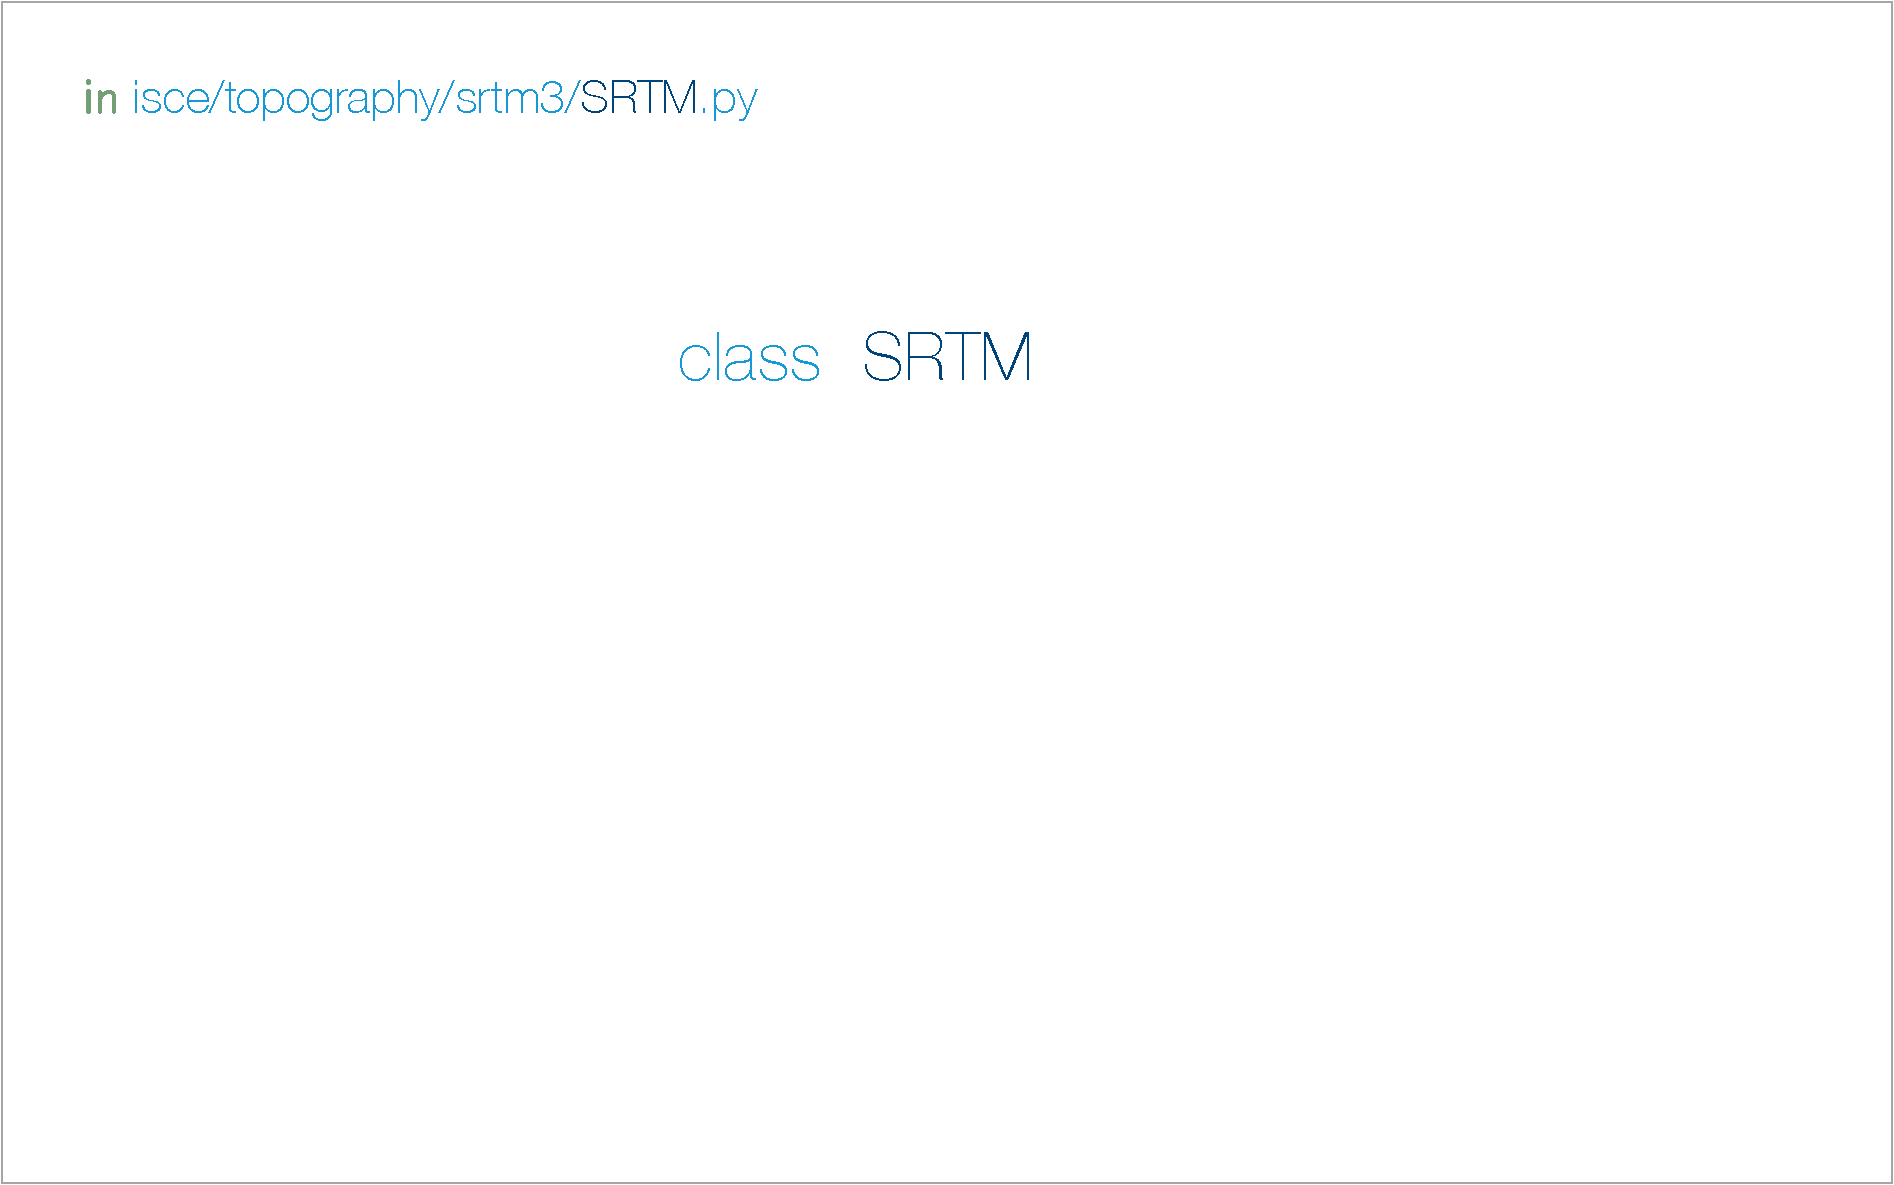
\includegraphics[width=1.0\textwidth]{component-package}}
    \only<2->{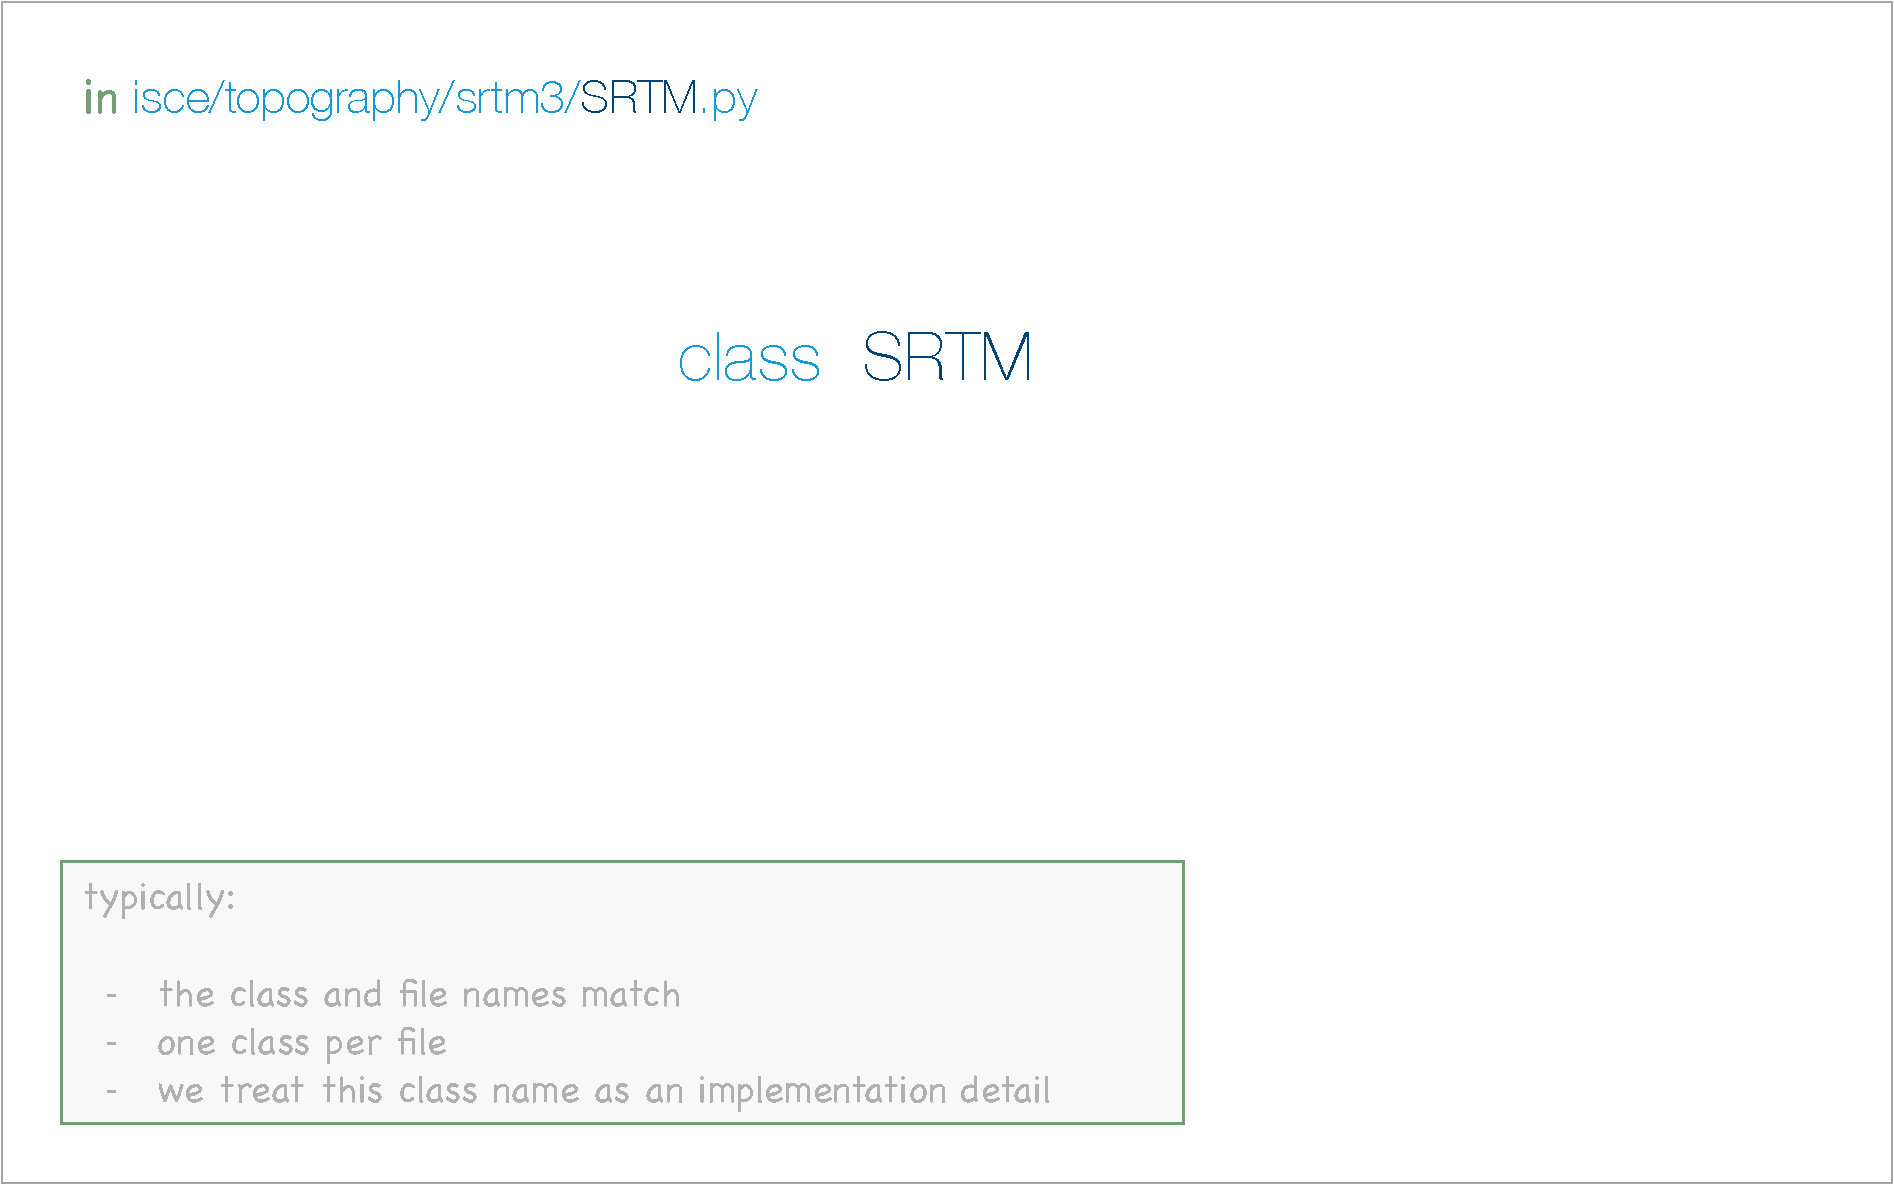
\includegraphics[width=1.0\textwidth]{component-package-explained}}
  \end{center}
%
\end{frame}

%-----------------------------------
\begin{frame}
%
  \frametitle{SRTM -- pedigree}
%
  \begin{center}
    \only<1>{
\includegraphics[width=1.0\textwidth]{component-base}}
    \only<2>{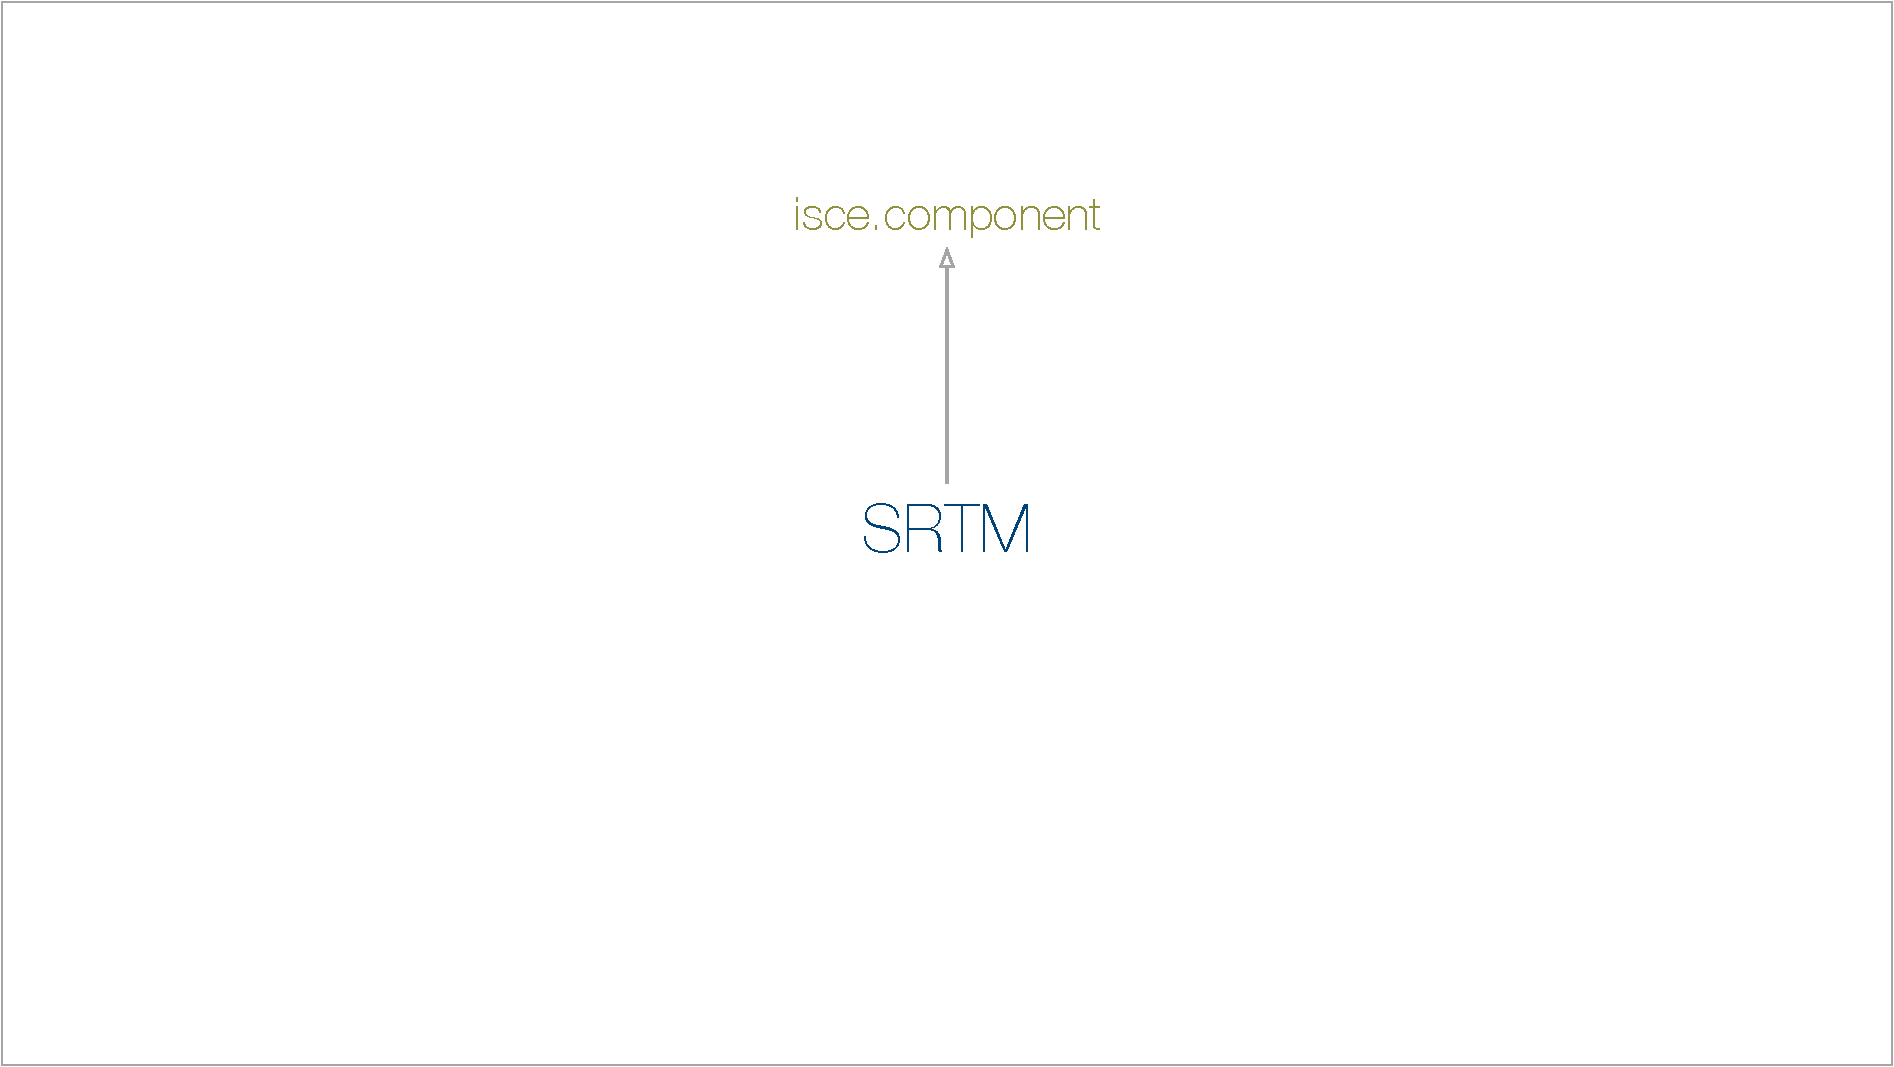
\includegraphics[width=1.0\textwidth]{component-inheritance}}
    \only<3>{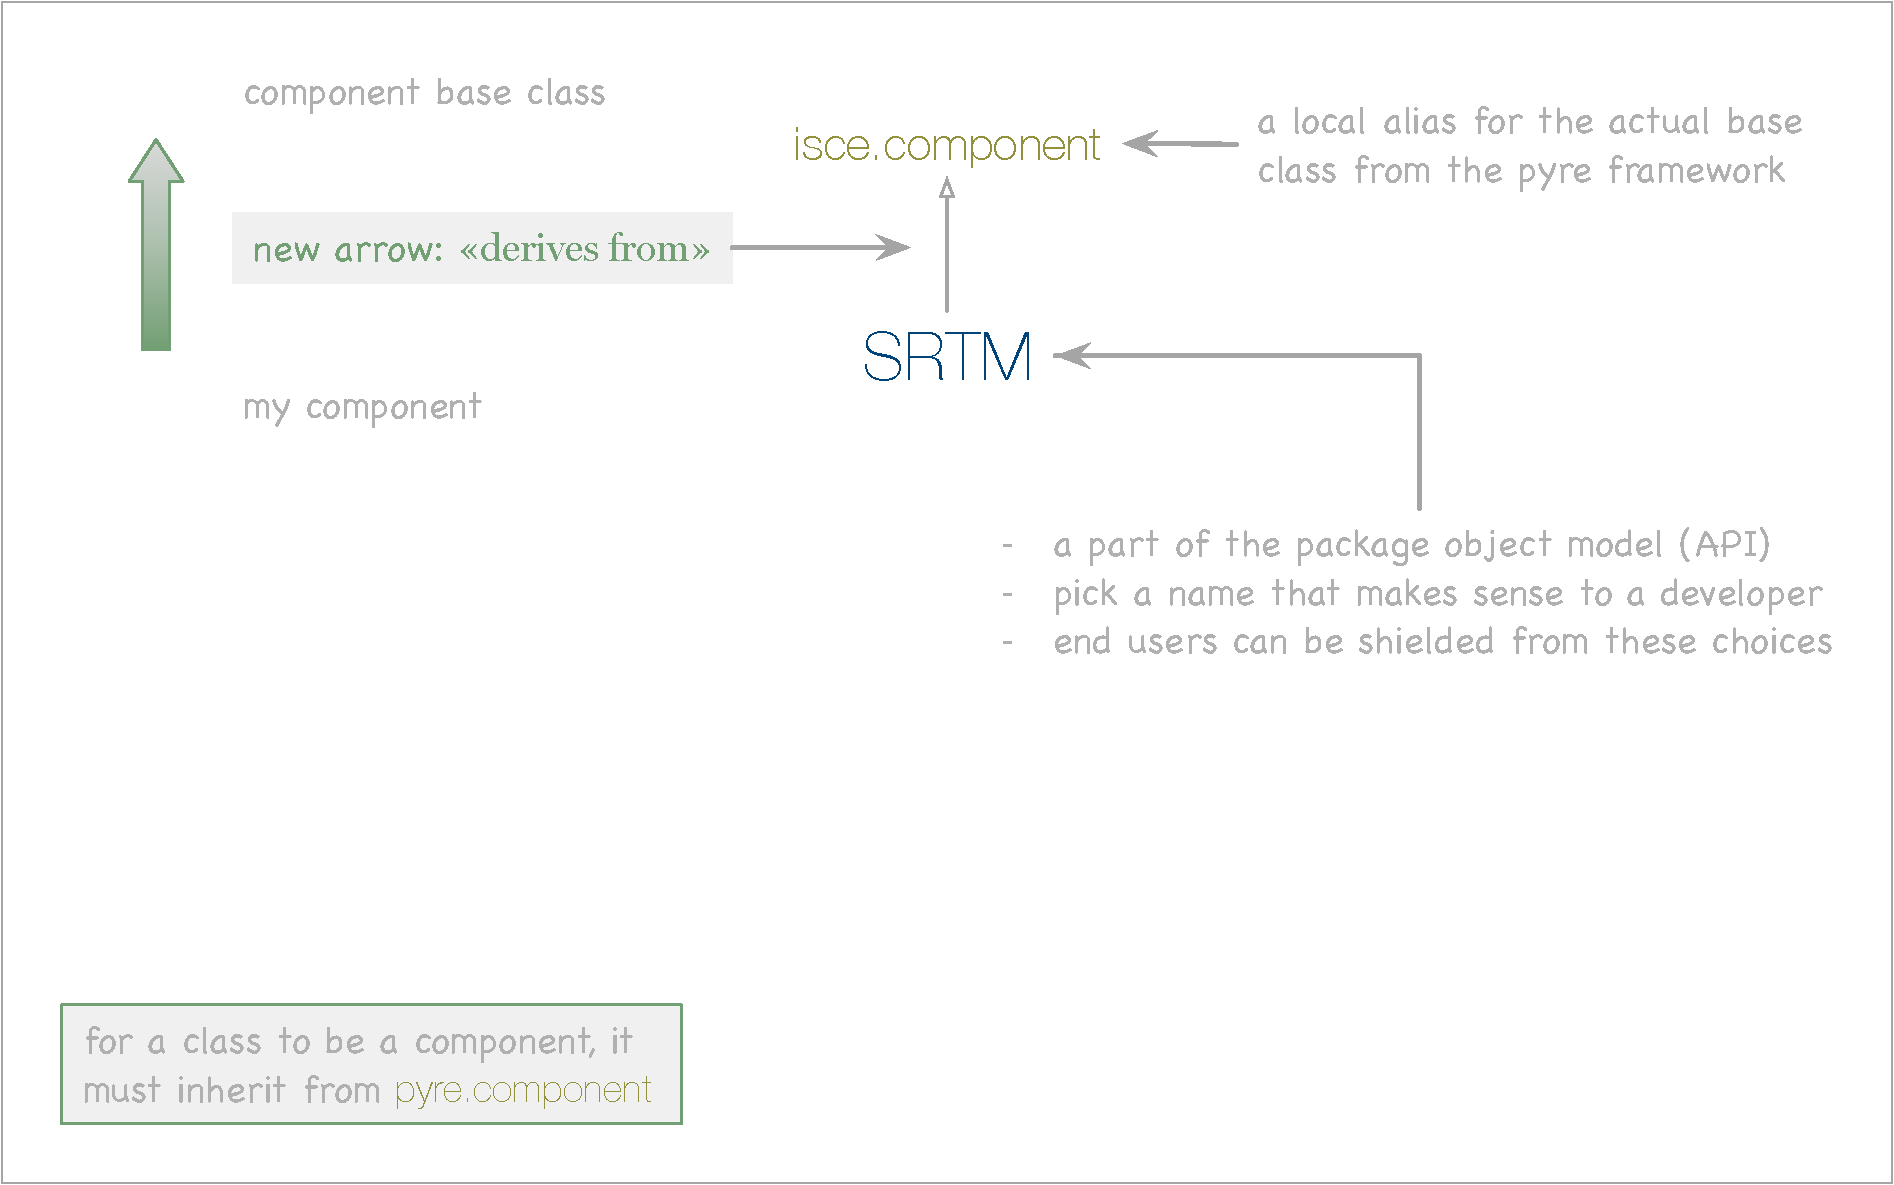
\includegraphics[width=1.0\textwidth]{component-inheritance-explained}}
  \end{center}
%
\end{frame}

%-----------------------------------
\begin{frame}[fragile]
%
  \frametitle{Component declaration}
%
  \vskip -3ex
  \begin{itemize}
%
  \item the instruction
    \begin{center}
      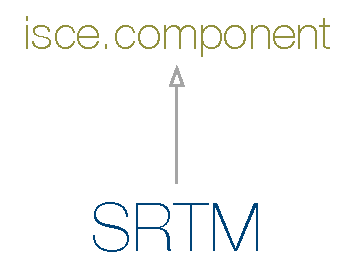
\includegraphics[height=10ex]{srtm-pedigree}
    \end{center}
%
  \item implies that instead of
%
    \begin{ipython}{}
class SRTM:
    """
    Access the SRTM data archive to download tiles and produce
    a digital elevation model for a specified region of interest
    """
    \end{ipython}
%
  \item we have to import the \isce\ package and derive from \class{isce.component}:
    \begin{ipython}{}
# support
import isce

# the srtm component
class SRTM(isce.component):
    """
    Access the SRTM data archive to download tiles and produce
    a digital elevation model for a specified region of interest
    """
    \end{ipython}
%
  \end{itemize}
%
\end{frame}

% --------------------------------------
% properties
\begin{frame}[fragile]
%
  \frametitle{Specifying the tile resolution}
%
  \begin{itemize}
%
  \item version 3 \srtm\ tiles come in two resolutions
%
    \begin{ipython}[firstnumber=4]{}
# the srtm component
class SRTM(isce.component):
    """
    Access the SRTM data archive to download tiles and produce
    a digital elevation model for a specified region of interest
    """

    # user configurable state
    resolution = 1 # arc seconds per pixel

    \end{ipython}
%
  \item how do we read the value of \trait{resolution} from a configuration file?
%
    \begin{ipfg}{}
      srtm:
          resolution = 1 ; arc seconds per pixel
    \end{ipfg}
%
    or, equivalently, from the command line of some driver script?
%
    \begin{ish}{}
      dem.py --srtm.resolution=1
    \end{ish}
%
  \item and resolve conflicts when different sources specify different values?
%
  \end{itemize}
%
\end{frame}

% --------------------------------------
% properties
\begin{frame}
%
  \frametitle{Components have properties}
%
  \begin{center}
    \only<1>{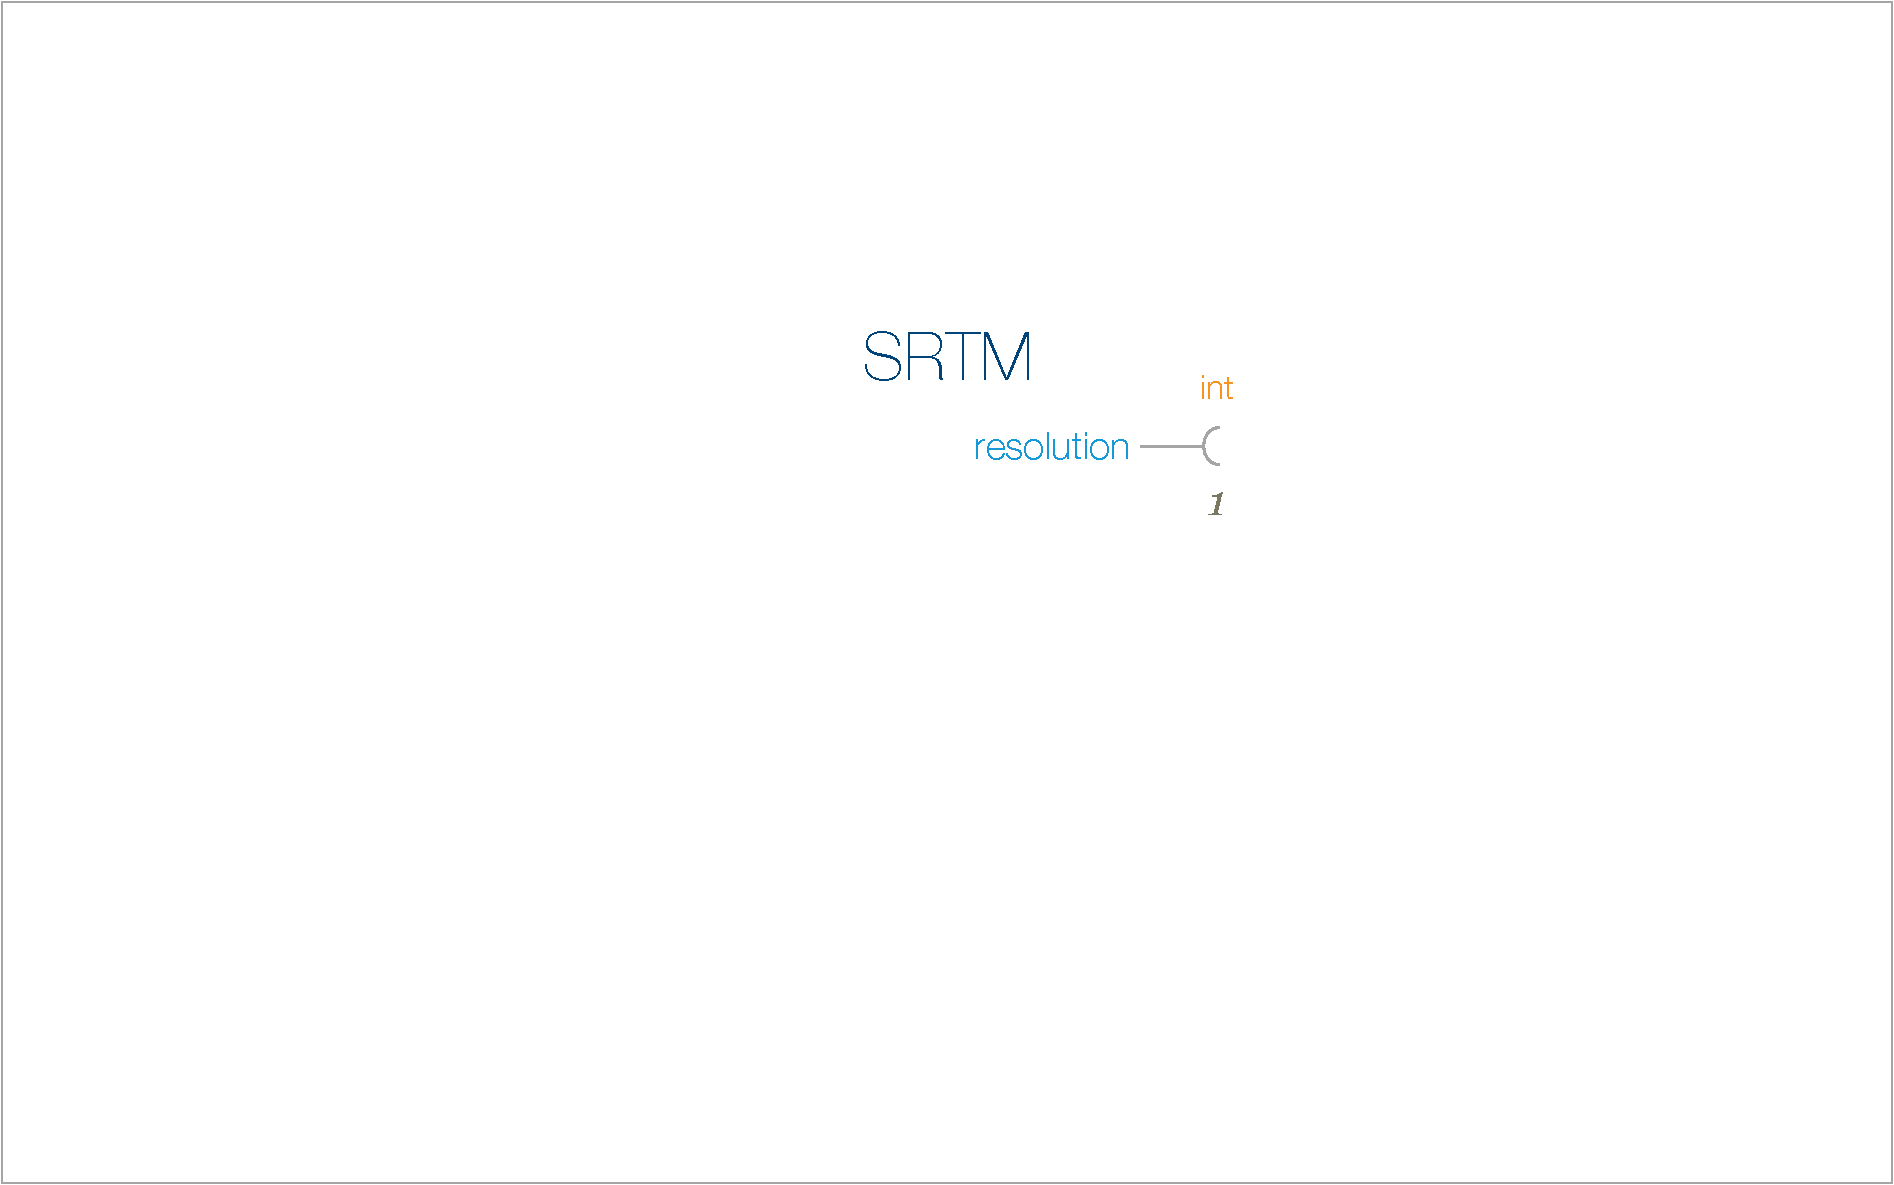
\includegraphics[width=1.0\textwidth]{component-properties}}
    \only<2->{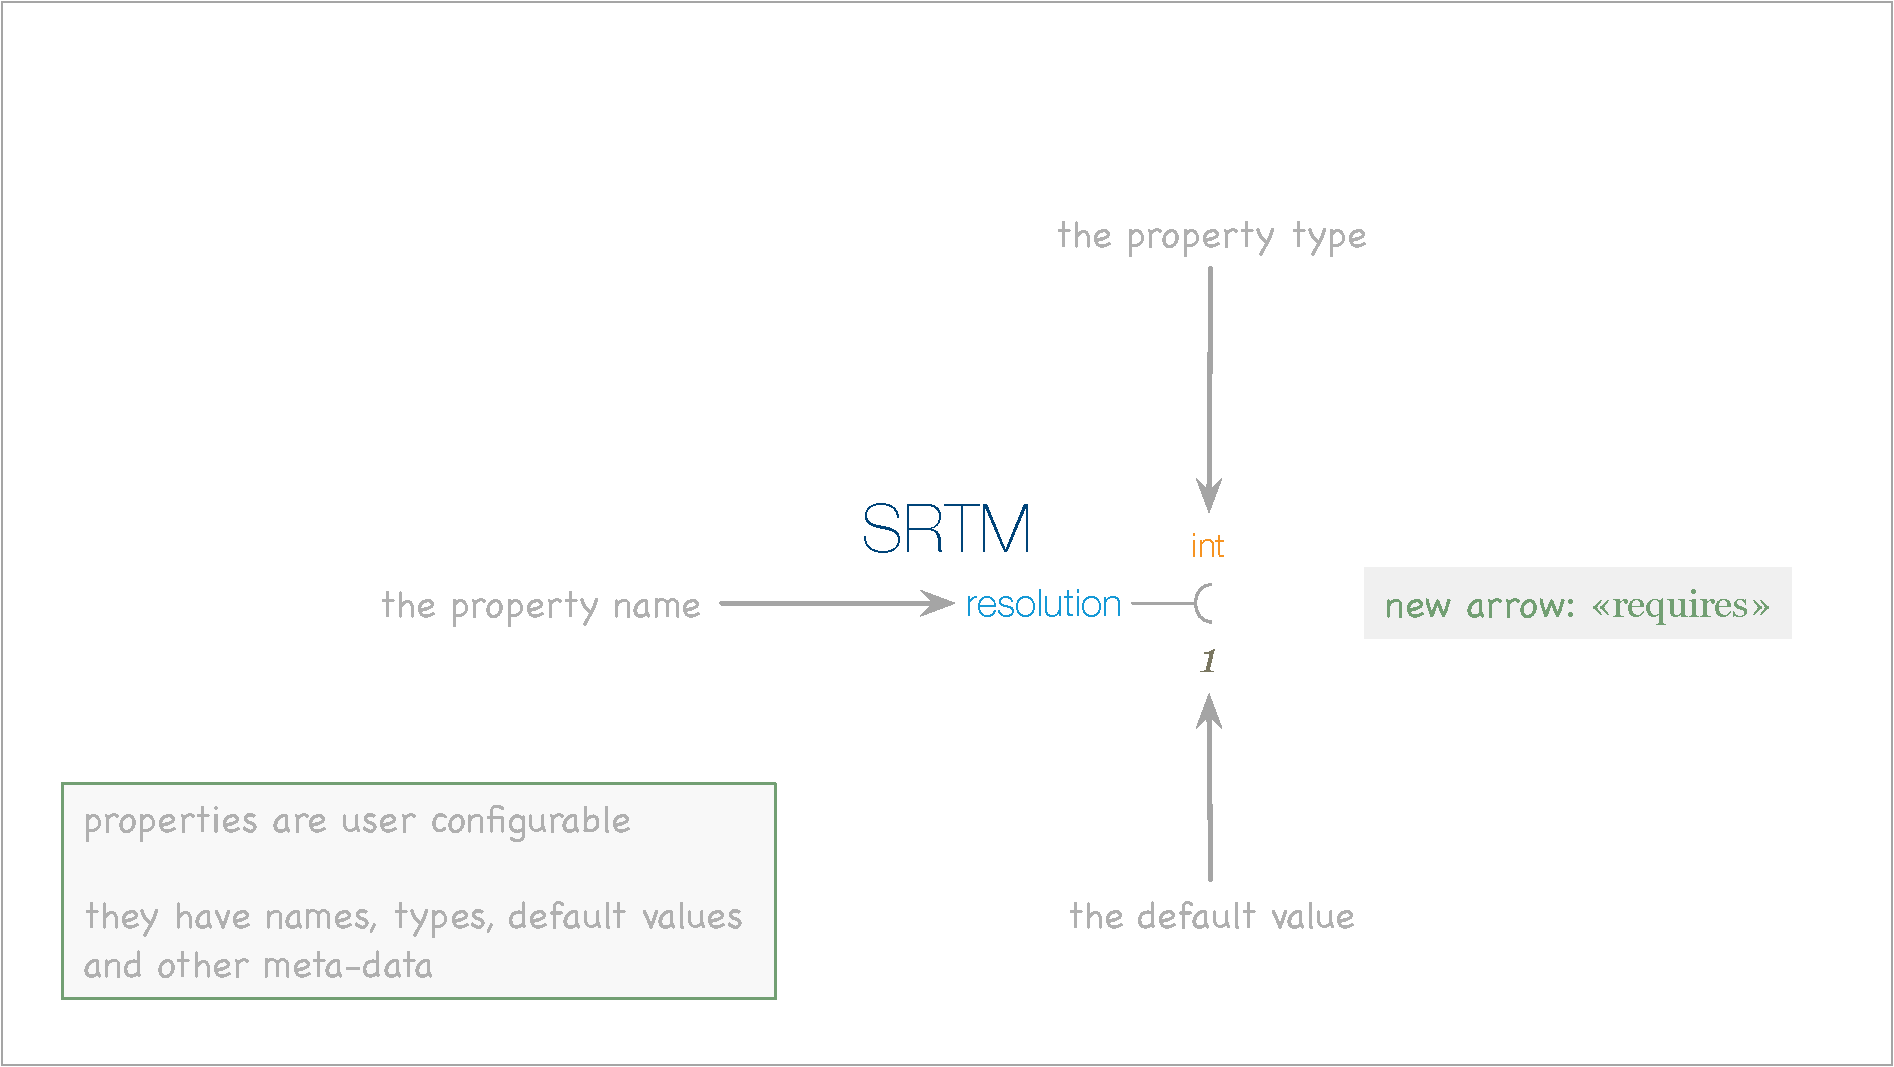
\includegraphics[width=1.0\textwidth]{component-properties-explained}}
  \end{center}
%
\end{frame}

% --------------------------------------
\begin{frame}[fragile]
%
  \frametitle{Adding properties to a component}
%
  \begin{itemize}
%
  \item the instruction
%
    \begin{center}
      
\includegraphics[height=10ex]{srtm-resolution}
    \end{center}
%
  \item it implies the following modification to the \class{SRTM} declaration:
%
    \begin{ipython}[firstnumber=4]{}
# the srtm component
class SRTM(isce.component):
    """
    Access the SRTM data archive to download tiles and produce
    a digital elevation model for a specified region of interest
    """

    # user configurable state
    resolution = isce.properties.int(default=1)
    resolution.doc = 'the tile resolution in arc seconds per pixel'

    \end{ipython}
%
  \item this states that \srtm\ requires that an \class{int} must be bound to the property
    \trait{resolution} at runtime, and if no suitable biding is provided, the default value of
    $1$ will be used
%
  \end{itemize}
%
\end{frame}

% --------------------------------------
\begin{frame}
%
  \frametitle{Properties}
%
  \vskip -2ex
  \begin{itemize}
%
  \item properties make sense for both classes and instances
    \begin{itemize}
    \item the class holds the default value that gets used in case the component instance does
      not have explicit configuration
    \item each instance gets its own private value when it gets configured
    \item the behavior is identical to regular python attributes
    \end{itemize}
%
  \item there is support for
    \begin{itemize}
    \item simple types: \function{bool}, \function{int}, \function{float}, \function{str}
    \item containers: \function{tuple}, \function{list}, \function{set}, \function{array}
    \item higher level: \function{date}, \function{time}, \function{istream},
      \function{ostream}, \function{inet}
    \item units: \function{dimensional}
    \item easy enough to implement your own; the requirements are very simple
    \end{itemize}
%
  \item metadata:
    \begin{itemize}
    \item \identifier{doc} and \identifier{tip}: simple and short documentation strings
    \item \identifier{default}: the default value, in case the user doesn't supply one
    \item \identifier{converters}: a chain of preprocessors of the string representation
    \item \identifier{normalizers}: a chain of post-processors of the converted value
    \item \identifier{validators}: a tuple of predicates that get called to ensure the property
      value satisfies the specified constraints
    \item you can add your own; the framework passes them through to your component
    \end{itemize}
%
  \end{itemize}
%
\end{frame}

% --------------------------------------
% units
\begin{frame}[fragile]
%
  \frametitle{Units}
%
  \vskip -2ex
  \begin{itemize}
%
  \item \function{dimensional} properties have units
%
  \item the low level support is in \package{pyre.units}
    \begin{itemize}
    \item full support for all SI base and derived units
    \item all common abbreviations and names from alternative systems of units
    \item correct arithmetic; proper handling of functions from \package{math}
    \end{itemize}
%
  \item consider
    \begin{ipython}{}
from math import cos
from pyre.units.SI import meter, second, radian

A = 2.5 * meter
t = 1.5 * second
ω = 4.2 * radian/second

x = A * cos(ω * t)
     \end{ipython}
%
   \item if the units in the argument to \function{cos} do not cancel, leaving a pure
     \keyword{float} behind, an exception is raised; \identifier{x} has dimensions of meters
%
  \end{itemize}
%
\end{frame}

%-----------------------------------
\begin{frame}
%
  \frametitle{SRTM -- family}
%
  \begin{center}
    \only<1>{
\includegraphics[width=1.0\textwidth]{component-family}}
    \only<2>{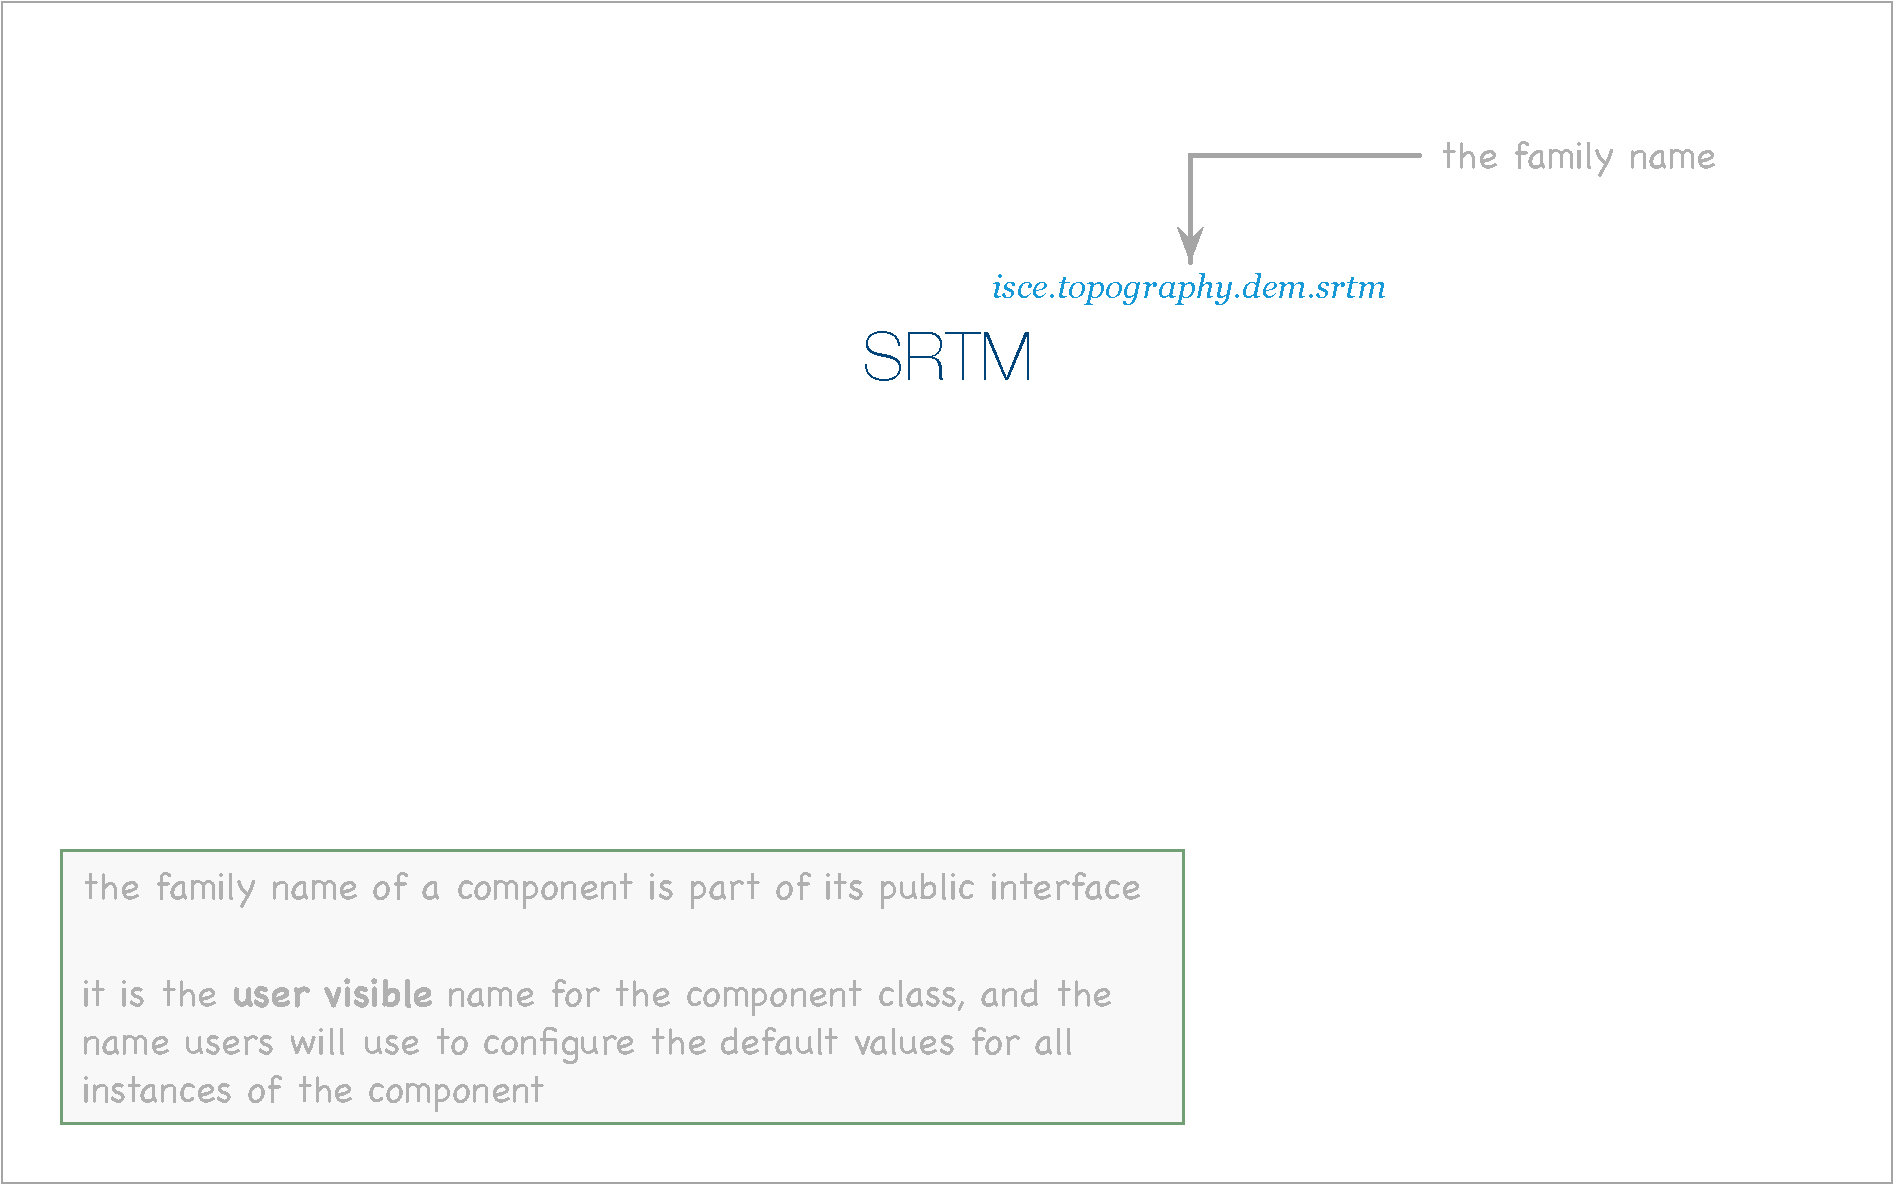
\includegraphics[width=1.0\textwidth]{component-family-explained}}
  \end{center}
%
\end{frame}

%-----------------------------------
\begin{frame}
%
  \frametitle{SRTM - protocol}
%
  \begin{center}
    \only<1>{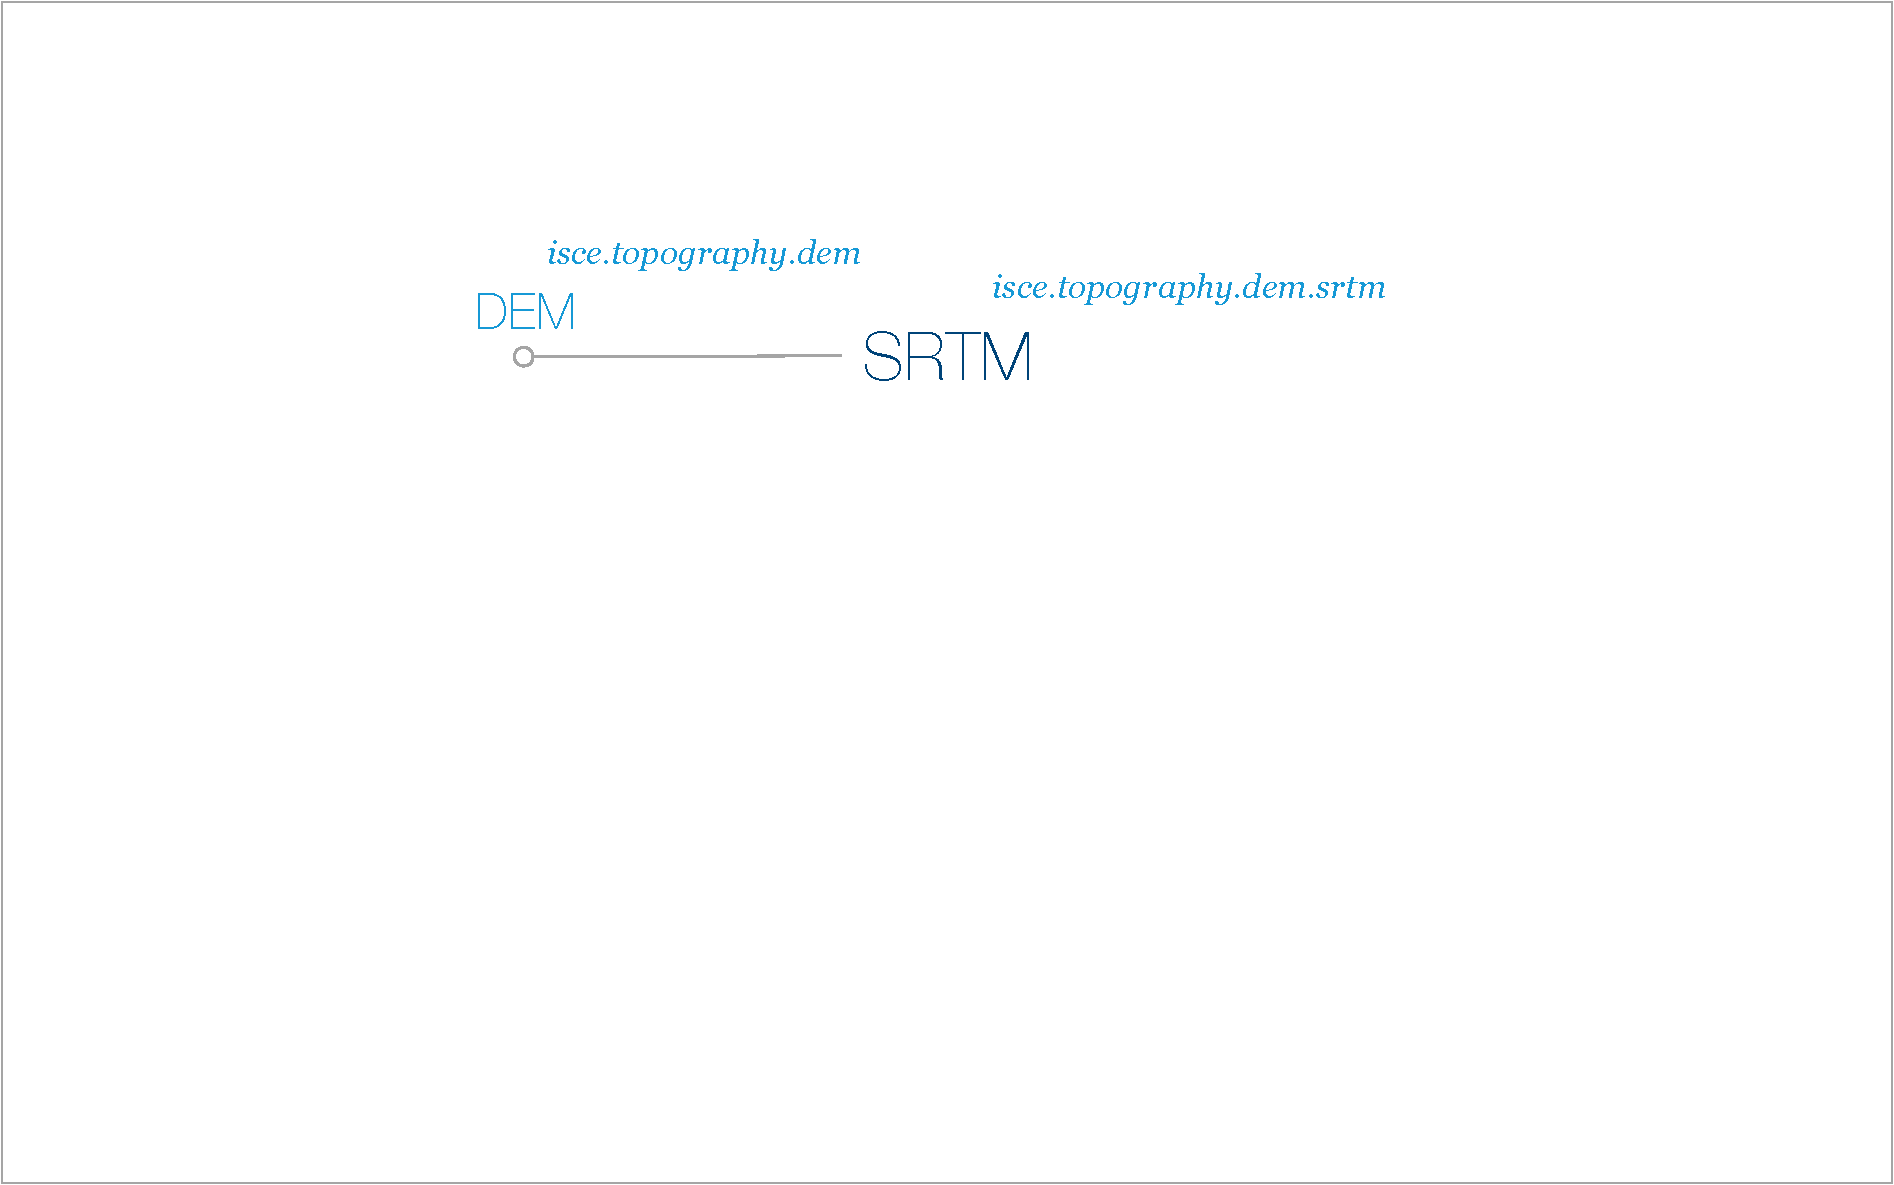
\includegraphics[width=1.0\textwidth]{component-implements}}
    \only<2>{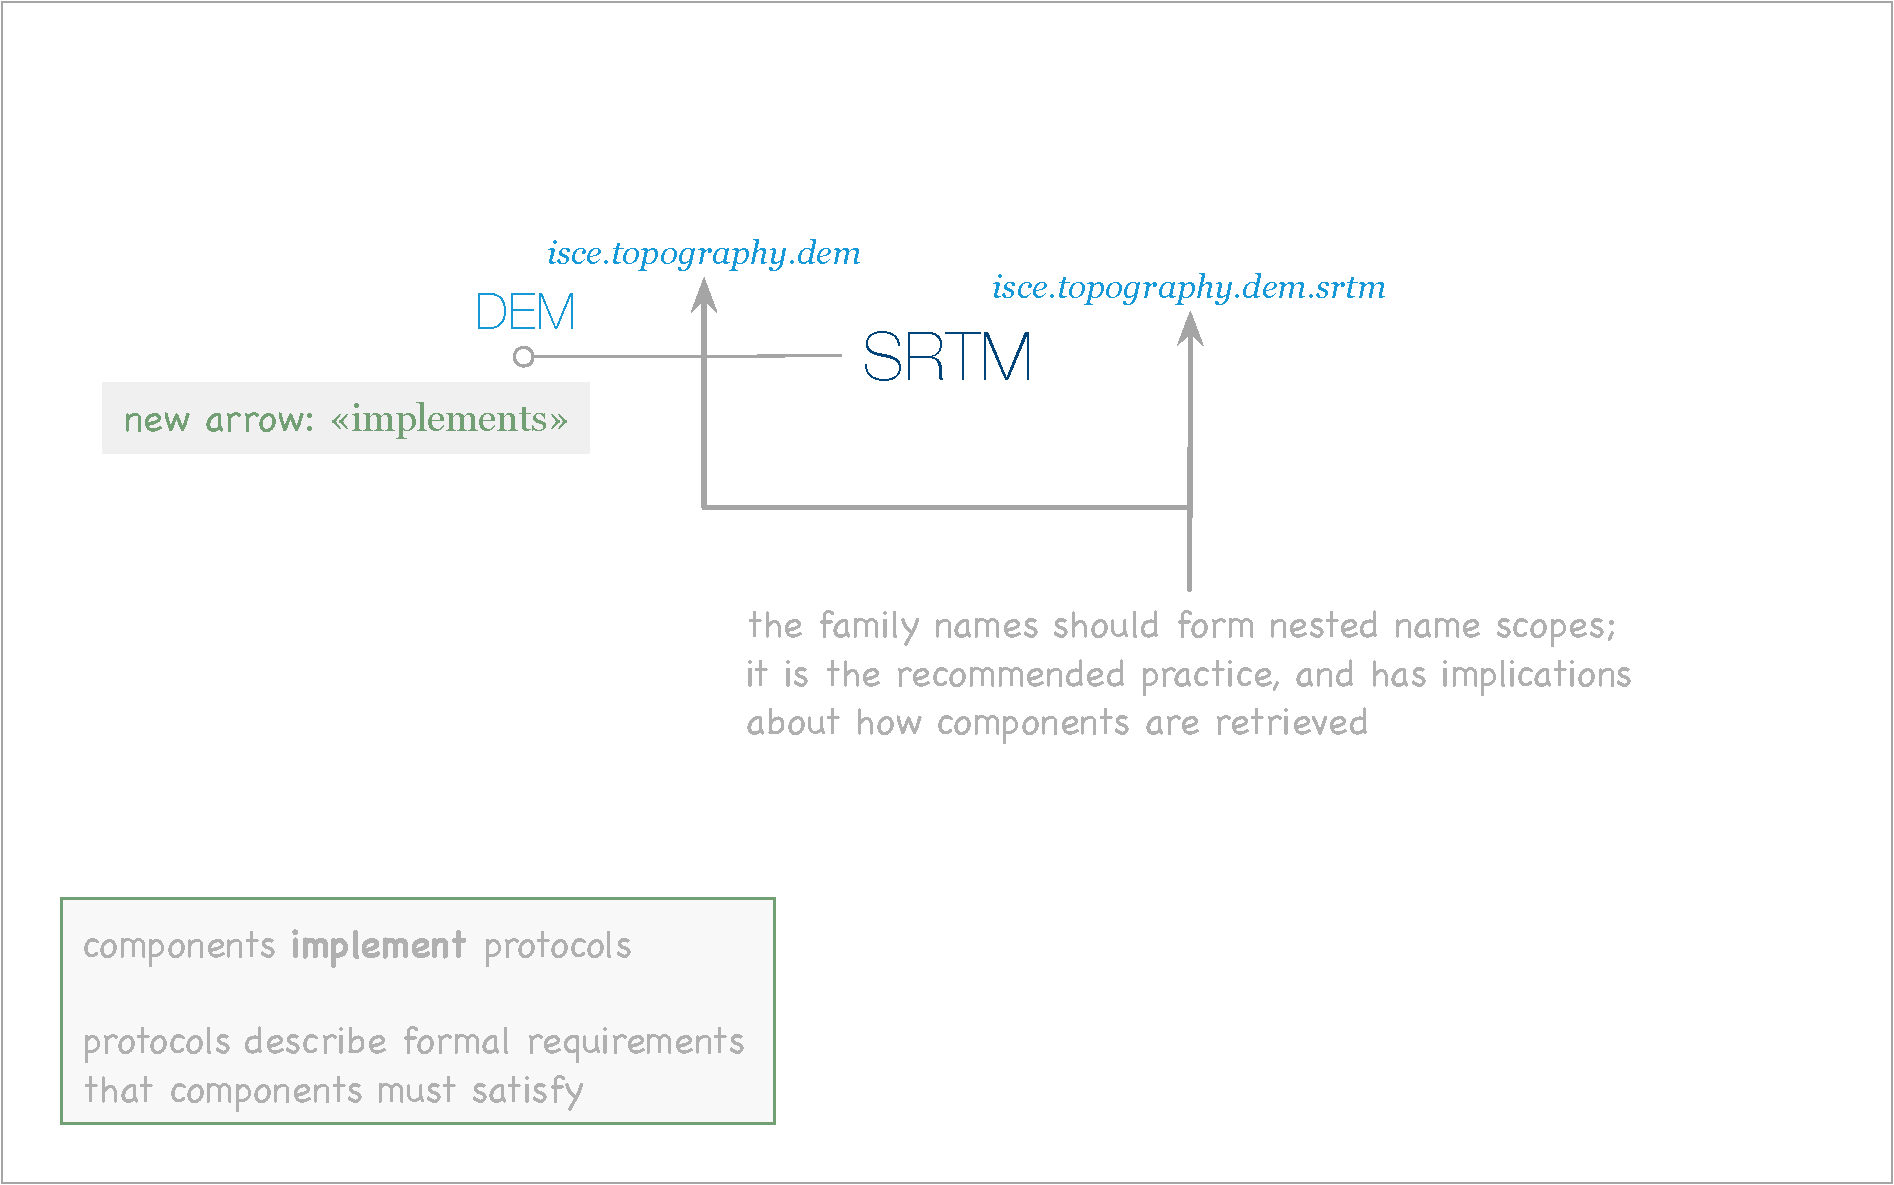
\includegraphics[width=1.0\textwidth]{component-implements-explained}}
  \end{center}
%
\end{frame}

% --------------------------------------
% recap
\begin{frame}
%
  \frametitle{Recap: what we know so far}
%
  \begin{itemize}
%
  \item \pyre\ components are evolved python objects
    \begin{itemize}
    \item the classes have family names, the instances have names
    \item these names are unique strings in hierarchical namespaces delimited by periods
    \item collections of components form packages \emph{implicitly}, based on the topmost level
      in their namespace
    \end{itemize}
%
  \item components have properties that are under the control of the \emph{user}
    \begin{itemize}
    \item they look and behave like regular attributes
    \item they are \emph{typed} to enable conversions from strings
    \item they have default values and other metadata
    \end{itemize}
%
  \item configuration is partly about assigning values to component properties
    \begin{itemize}
    \item a requirement for supporting user interfaces
    \item intuitive syntax for the command line
    \item simple configuration files in a variety of formats: \identifier{XML}, Microsoft
      Windows \identifier{.ini}, native \identifier{.pfg}
    \end{itemize}
%
  \item configuration is automatically handled by the framework and requires no explicit
    involvement on the part of the component author
%
  \end{itemize}
%
\end{frame}

% --------------------------------------
\begin{frame}
%
  \frametitle{Components and protocols}
%
  \begin{itemize}
%
  \item a design pattern\supercite{patterns} that enables the assembly of applications out of
    interchangeable parts, under the control of the end user
      \begin{itemize}
      \item \emph{protocols} are abstract specifications of application requirements
      \item \emph{components} are concrete implementations that satisfy requirements
      \end{itemize}
%
    \item protocols make it possible to write applications without any \emph{a priori} knowledge
      of implementation specifics
%
    \item inversion of control\supercite{johnson-88}:
      \begin{itemize}
      \item the binding of actual implementations to the application requirements happens at
        runtime, under the control of the end user
      \end{itemize}
%
    \item in \pyre, the user
      \begin{itemize}
      \item controls the application state through configuration files, the user interface, the
        command line
      \item specifies components using simple URIs
      \end{itemize}
%
    \item the goal is to isolate contributors from each other as much as possible, and provide
      a coherent and usable strategy for composing non-trivial applications
%
  \end{itemize}
%
\end{frame}

%%% Local Variables:
%%% mode: latex
%%% TeX-master: "../pyre"
%%% End:

% end of file

% -*- LaTeX -*-
% -*- coding: utf-8 -*-
%
% michael a.g. aïvázis <michael.aivazis@para-sim.com>
% (c) 2003-2017 all rights reserved
%

\section{applications}

% --------------------------------------
\subsection{simple}
\begin{frame}[fragile]
  \label{frame:applications-simple}
%
  \frametitle{A simple application script}
%
  \vskip -3ex
  \begin{itemize}
%
  \item \component{Stitcher}, a simple \pyrebuiltin{isce.application}
%
    \python{}{listings/stitch.py}
%
  \end{itemize}
%
\end{frame}

% --------------------------------------
\begin{frame}
%
  \frametitle{Applications as component containers}
%
  \begin{itemize}
%
  \item in \lstlineref{applications-simple-decl}, \component{Stitcher} derives from
    \pyrebuiltin{isce.application}
    \begin{itemize}
    \item which makes it a component; see \frameref{applications-plexus-pedigree} for its
      pedigree
    \item with some special capabilities
    \end{itemize}
%
  \item in \lstlineref{applications-simple-dem}, \component{Stitcher} registers a requirement
    for a \protocol{dem} compatible implementation
    \begin{itemize}
    \item note the use of the protocol as the type of the trait
    \item the syntax is the same as for properties
    \item no explicit default is provided, so the protocol will be asked to provide one in the
      event that the user does not express a preference
    \end{itemize}
%
  \item the special behavior \method{main} in \lstlineref{applications-simple-main} is the
    application entry point
    \begin{itemize}
    \item it is invoked by the framework after the application instance is configured
    \end{itemize}
%
  \item the stanza after \lstlineref{applications-simple-boot} bootstraps the application:
    \begin{itemize}
    \item an instance is created and named
    \item the framework searches for a configuration file named after the instance
    \item the app is launched by invoking the method \method{run}
    \item the framework determines the hosting strategy based on the user's choice of
      application shell; the full details are on \frameref{applications-plexus-pedigree}
    \item it invokes the method \method{main} and collects the return status
    \item the status is shared with the user's environment by asking python to terminate in a
      controlled way
    \end{itemize}
%
  \end{itemize}
%
\end{frame}

% --------------------------------------
\subsection{configuration}
\begin{frame}
%
  \frametitle{Exercising the default configuration}
%
  \vskip -3ex
  \begin{itemize}
%
  \item let's focus on the relationship between \instance{stitch} and its trait \trait{dem}
%
  \item by the time we invoke the method \method{stitch} on
    \lstlineref{applications-simple-stitch}, we expect a fully configured instance of some
    component compatible with \protocol{isce.topography.dem}
%
  \item compatibility with the protocol guarantees that
    \begin{itemize}
    \item we have a way of specifying the region of interest
    \item the method \method{stitch} exists
    \end{itemize}
    since both of these are \protocol{isce.topography.dem} requirements
%
  \item if we provide no configuration
    \begin{itemize}
    \item evaluation of \literal{self.dem} will initiate a search for a suitable candidate
    \item the protocol will be asked to provide a default value, which will return the class
      record of \component{SRTM}
    \item since \component{SRTM} is assignment compatible with \protocol{isce.topography.dem},
      the framework will accept it as a viable candidate and configure it
    \item the framework will initiate the process of creating and configuring an instance with
      the name \literal{stitch.dem}, to match the name of the \component{Stitcher} property
    \item the instance will become the value of \literal{self.dem} for our application instance
    \item the method \method{stitch} will be invoked and find \trait{region} set to an empty
      \schema{array}, and \trait{resolution} set to \defaultvalue{1}
    \end{itemize}
%
  \item this is a typical strategy: by default, the app will function correctly but will not do
    much
%
  \end{itemize}
%
\end{frame}

% --------------------------------------
\begin{frame}
%
  \frametitle{The application inventory}
%
  \vskip -3ex
  \begin{itemize}
%
  \item let's summarize what is and is not configurable
    \begin{itemize}
    \item the \component{Stitcher} class declaration on \lstlineref{applications-simple-decl}
      does not specify a family name; \component{Stitcher} is not a public class, and there is
      no way to alter the settings for the class-wide defaults
    \item our application instance was given a name in the bootstrapping stanza after
      \lstlineref{applications-simple-boot}, so its \trait{dem} is under our control; it is
      accessible as \trait{stitch.dem}
    \item the \component{SRTM} class declaration has a family, so we can control the default
      values for \trait{region} and \trait{resolution} for all its instances; their names are
      \begin{itemize}
      \item \trait{isce.topography.dem.srtm.region}
      \item \trait{isce.topography.dem.srtm.resolution}
      \end{itemize}
      respectively (see \frameref{components-public})
    \item the \component{SRTM} instance that is bound to our application instance is accessible
      as \trait{stitch.dem}; hence its \trait{region} and \trait{resolution} values are
      accessible as
      \begin{itemize}
      \item \trait{stitch.dem.region}
      \item \trait{stitch.dem.resolution}
      \end{itemize}
      respectively (again, see \frameref{components-public})
    \end{itemize}
%
  \end{itemize}
%
\end{frame}

% --------------------------------------
\begin{frame}[fragile]
%
  \frametitle{Configuration from the command line}
%
  \vskip -3ex
  \begin{itemize}
%
  \item suppose that the code on \frameref{applications-simple} is in a script called
    \package{stitch.py}; we don't have an alternative implementation of
    \protocol{isce.topography.dem}, but we can be explicit about the one we have
    \begin{ish}[gobble=4, numbers=none]{}
      ~/tmp> stitch.py --stitch.dem=isce.topography.dem.srtm
    \end{ish}
%
  \item application traits are automatically available at the top level of the namespace, so we
    can shorten this to
    \begin{ish}[gobble=4, numbers=none]{}
      ~/tmp> stitch.py --dem=isce.topography.dem.srtm
    \end{ish}
%
  \item we can take advantage of the rational organization of the \isce\ namespace to
    shorten this further
    \begin{ish}[gobble=4, numbers=none]{}
      ~/tmp> stitch.py --dem=srtm
    \end{ish}
%
\item we can also control any property of \trait{dem}
    \begin{ish}[gobble=4, numbers=none]{}
      ~/tmp> stitch.py --dem=srtm --dem.resolution=3
    \end{ish}
%
  \item mistakes are flagged
    \begin{ish}[gobble=4, numbers=none]{}
      ~/tmp> stitch.py --dem=madeup
      stitch: could not resolve 'madeup' into a component that implements
      protocol 'isce.topography.dem'
    \end{ish}
%
  \item the right hand side of the \trait{dem} assignment has a very rich syntax and is a
    critical part of the extensibility of our applications
%
  \end{itemize}
%
\end{frame}

% --------------------------------------
\begin{frame}[fragile]
%
  \label{frame:applications-config}
%
  \frametitle{Application configuration files}
%
  \vskip -3ex
  \begin{itemize}
%
  \item settings that we expect to change less frequently can be placed in configuration files;
    let's adapt the sample from \frameref{srtm-pfg}
%
    \pfg{firstnumber=7, linerange={7-20}}{listings/stitch.pfg}
%
  \item the ability to capture the namespace hierarchy with the block structure makes for very
    readable configuration files
%
  \item the simplicity of the syntax helps as well
%
  \item there are many ways to force the framework to recognize these settings
    \begin{itemize}
    \item the natural one is to place them in a file called \package{stitch.pfg} in the working
      directory
    \item see \frameref{applications-config-sources} for a more complete picture
    \end{itemize}
%
  \end{itemize}
%
\end{frame}

% --------------------------------------
\begin{frame}
%
  \label{frame:applications-config-conditional}
%
  \frametitle{Conditional assignments}
%
  \vskip -3ex
  \begin{itemize}
%
  \item the settings on \frameref{applications-config} contain a subtle bug:
    \begin{itemize}
    \item setting \trait{region} is ok, since the \protocol{isce.topography.dem} forces all
      compatible implementations to have this trait
    \item but this is not the case with \trait{resolution}
    \end{itemize}
%
  \item an option is to set a default resolution for all instances of \component{SRTM}, but in
    general this is not the right solution; besides, it only works if every use of
    \component{SRTM} requires the high resolution tiles
%
  \item what we need is a way to express the following: if \trait{stitch.dem} is an instance of
    \component{isce.topography.dem.srtm}, then set \trait{resolution} to 1
%
  \item there is special syntax for this use case
    \pfg{firstnumber=7, linerange={7-18}}{listings/stitch-conditional.pfg}
%
  \item now the setting applies only when \trati{dem} is bound to an \component{SRTM} instance
%
  \end{itemize}
%
\end{frame}

% --------------------------------------
\begin{frame}
%
  \frametitle{Configuration event ranking}
%
  \vskip -3ex
  \begin{itemize}
%
  \item each configuration event is assigned a priority when it is encountered
    \begin{itemize}
    \item the priority is a pair: (category, collation sequence)
    \item the priority category is determined by the event source
    \item whether and event has an effect on the corresponding trait depends on the priority of
      the current value
    \item this way the framework can respond correctly to newly discovered information
    \end{itemize}
%
  \item the framework recognizes the following priority categories, in increasing order
%
    \begin{itemize}
%
    \item defaults: values from component trait declarations in the source code
      \begin{itemize}
      \item this is the developer's contribution
      \end{itemize}
%
    \item boot: assigned while the framework is booting
      \begin{itemize}
      \item currently, assigned to the values of user environment variables
      \end{itemize}
%
    \item package: values from configuration files in the install directory of a package
      \begin{itemize}
      \item this is the sysadmin's opportunity to configure a package for users on a given
        system
      \end{itemize}
%
    \item user: values from the user's configuration files, typically in \url{~/.pyre}
      \begin{itemize}
      \item this is the user's opportunity to override package settings
      \end{itemize}
%
    \item command line: the priority of values retrieved from the command line for the current
      invocation of the application
%
    \item explicit: direct assignments in user code
      \begin{itemize}
      \item in general, this is discouraged unless configuring a subcomponent
      \end{itemize}
%
    \item framework: a priority that essentially renders values as read-only
%
    \end{itemize}
%
  \end{itemize}
%
\end{frame}

% --------------------------------------
\begin{frame}
%
  \label{frame:applications-config-sources}
%
  \frametitle{Configuration event sources}
%
  \vskip -3ex
  \begin{itemize}
%
  \item configuration is a dynamic process in \pyre; it happens both explicitly, such as
    when processing the command line arguments, and implicitly, when encountering a new package
%
    \begin{itemize}
    \item compliant packages register themselves with the framework
    \item the framework forms a filename out of the package name and an extension from each
      register configuration codec
    \item a search over the locations on the \trait{configpath} is initiated
    \item all matching configuration files are loaded
    \end{itemize}
%
  \item by default, \trait{configpath} knows about the \pyre\ install location, the user's
    \url{.pyre} directory, and the current working directory
%
  \item this process cascades into the dependencies of each package
    \begin{itemize}
    \item for example, on \lstlineref{applications-simple-import} of
      \frameref{applications-simple}, we \keyword{import} \isce\, which in turn imports \pyre
    \item this means that a search for \literal{pyre.\{pfg,cfg,pml\}} is initiated, and every
      match is loaded
    \item followed by a search for \literal{isce.\{pfg,cfg,pml\}}
    \end{itemize}
%
  \item similarly, while building the application instance, the framework conducts a search for
    a configuration file derived out of the instance name, and loads any matches
    \begin{itemize}
    \item this is the preferred way to configure an application implicitly; the others are
      meant to modify the defaults from the source code
    \end{itemize}
%
  \item while processing the command line arguments
%
  \item by invoking the application with an \literal{-config} argument
%
  \item in user code, by invoking the function \function{loadConfiguration()} explicitly
%
  \end{itemize}
%
\end{frame}

% --------------------------------------
\subsection{integration}
\begin{frame}
%
  \frametitle{Providing help}
%
\end{frame}

% --------------------------------------
\subsection{plexus}
\begin{frame}
%
  \frametitle{\component{Plexus}: support for behavior rich applications}
%
\end{frame}

% --------------------------------------
\begin{frame}
%
  \frametitle{Application introspection: the action \action{about}}
%
\end{frame}

% --------------------------------------
\subsection{runtime}
\begin{frame}
%
  \frametitle{Framework services for applications}
%
\end{frame}

\begin{frame}
%
  \frametitle{Virtual filesystems}
%
\end{frame}

% --------------------------------------
\subsection{shells}
\begin{frame}
%
  \frametitle{The \component{script} shell}
%
\end{frame}

% --------------------------------------
\begin{frame}
%
  \frametitle{The \component{interactive} shell}
%
\end{frame}

% --------------------------------------
\begin{frame}
%
  \frametitle{The \component{web} shell}
%
\end{frame}

% --------------------------------------
\begin{frame}
%
  \label{frame:applications-plexus-pedigree}
%
  \frametitle{The \component{Plexus} structure}
%
  \vskip -3ex
  \only<1>{
    \begin{center}
      
\includegraphics[width=0.9\textwidth]{pyre-plexus-base}
    \end{center}
  }
  \only<2>{
    \begin{center}
      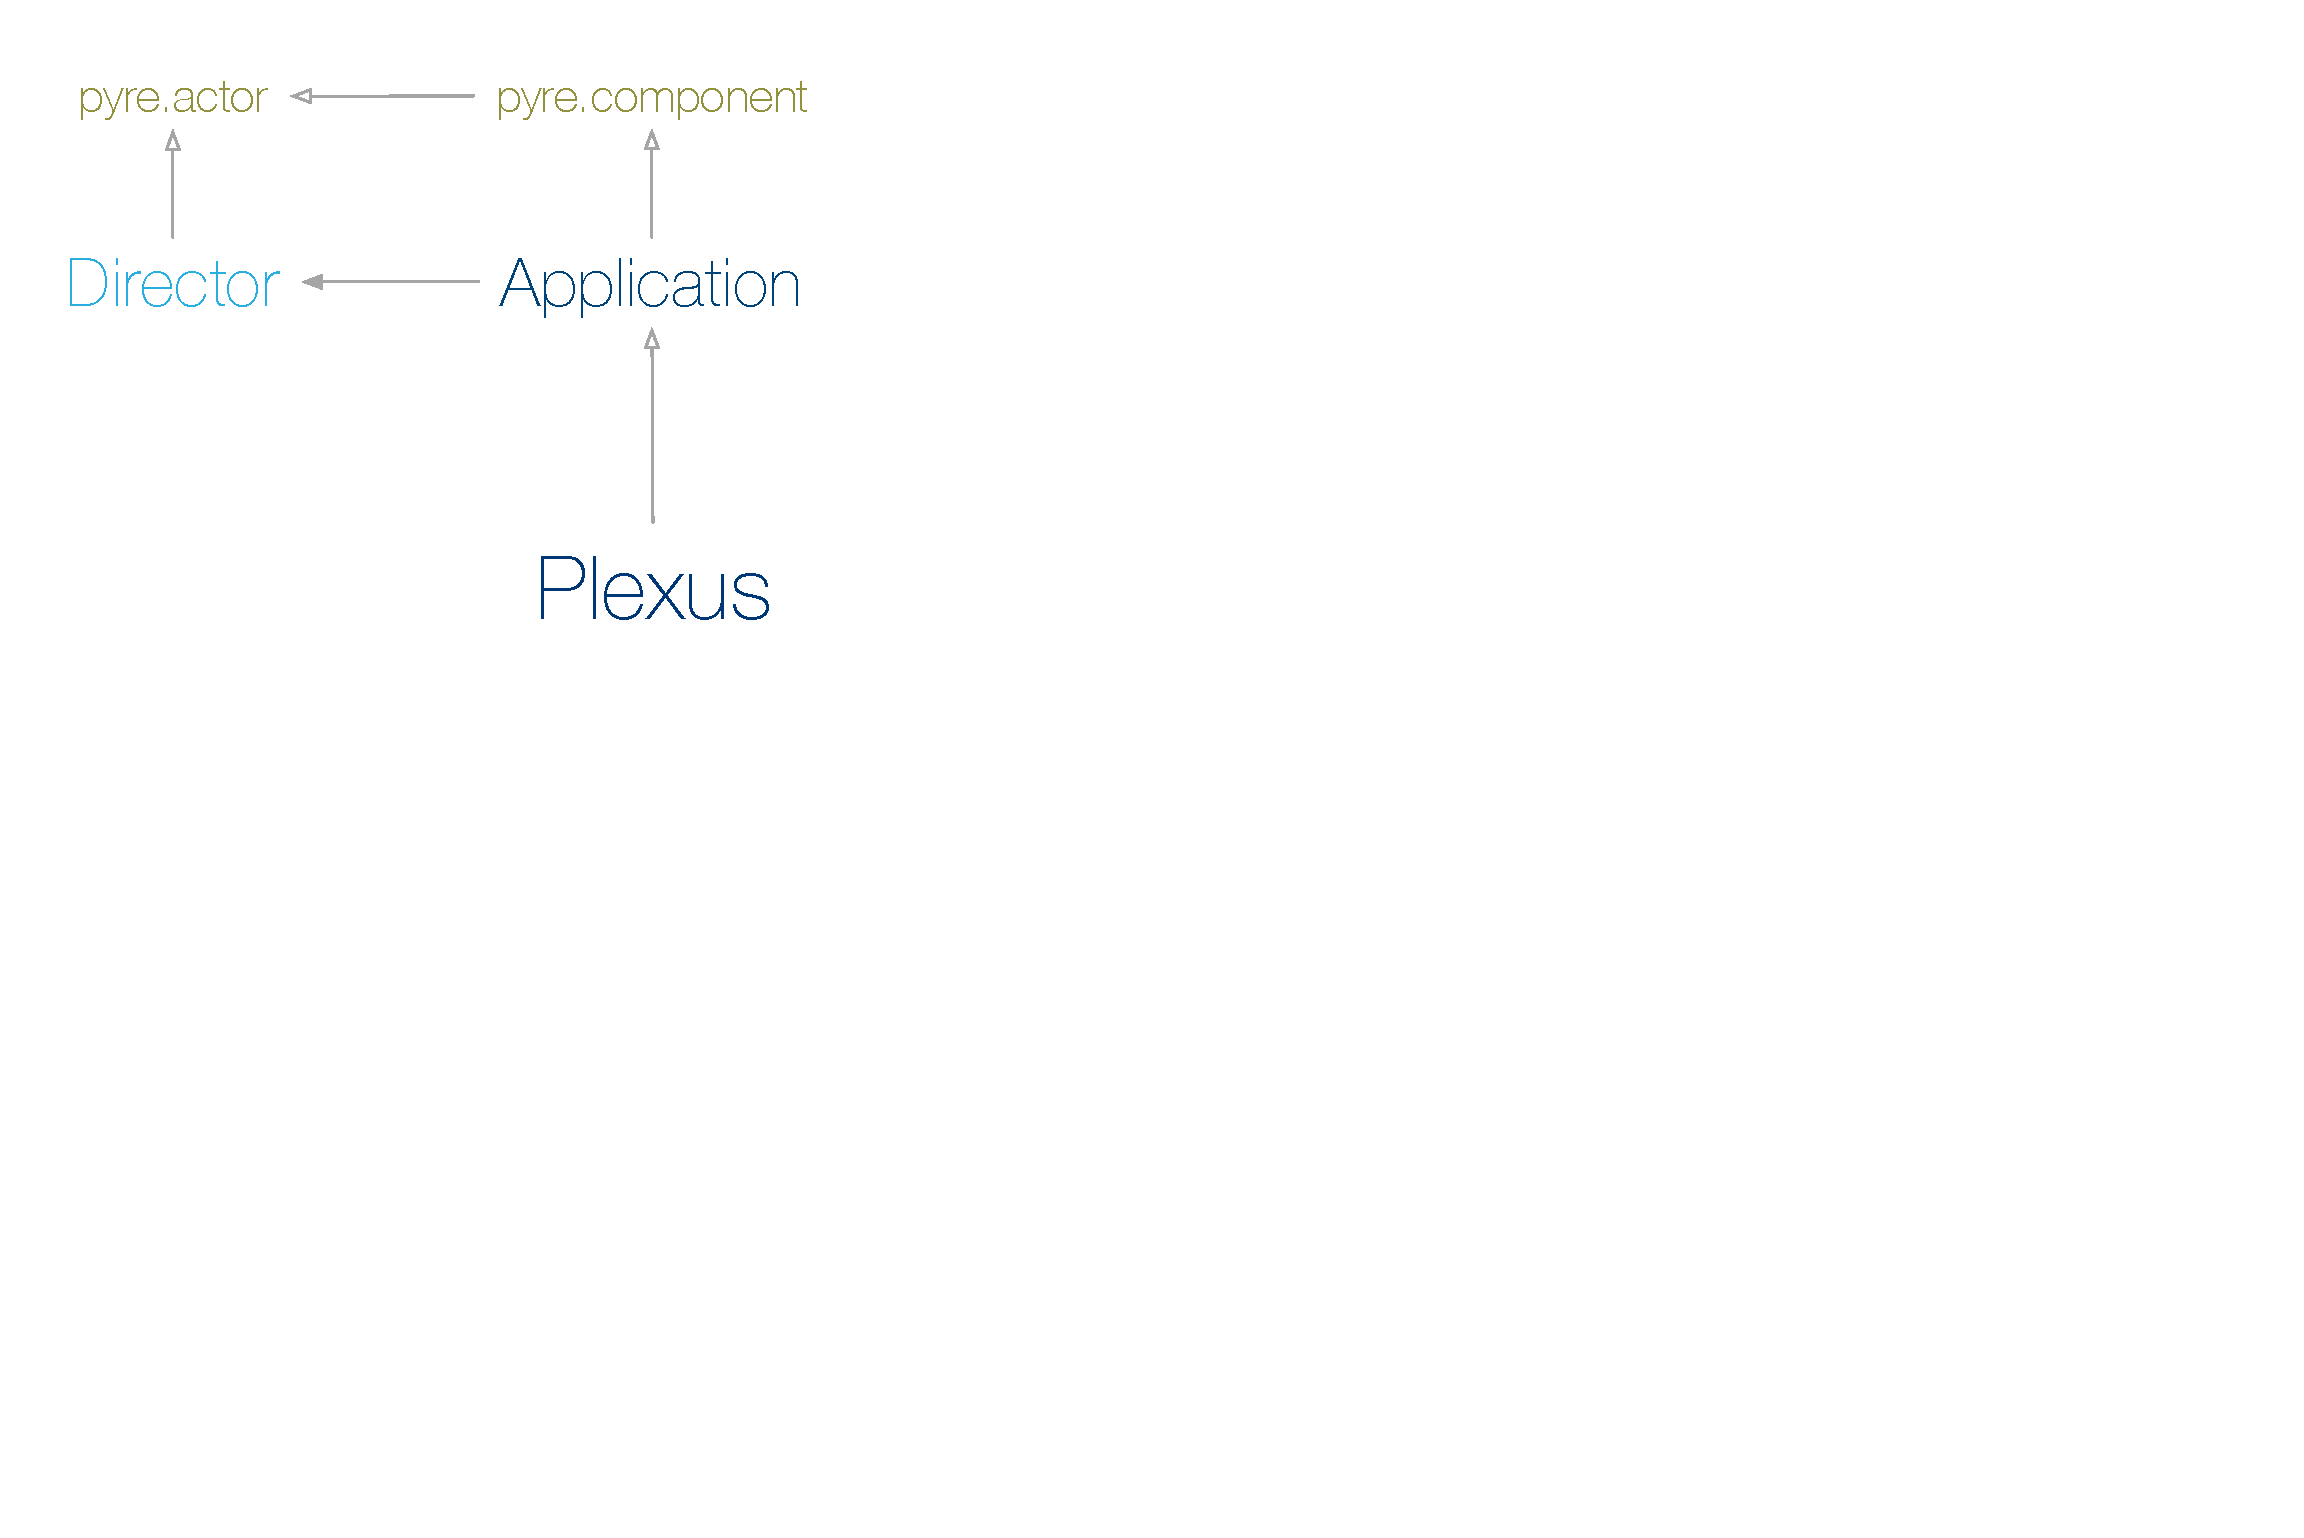
\includegraphics[width=0.9\textwidth]{pyre-plexus-pedigree}
    \end{center}
  }
  \only<3>{
    \begin{center}
      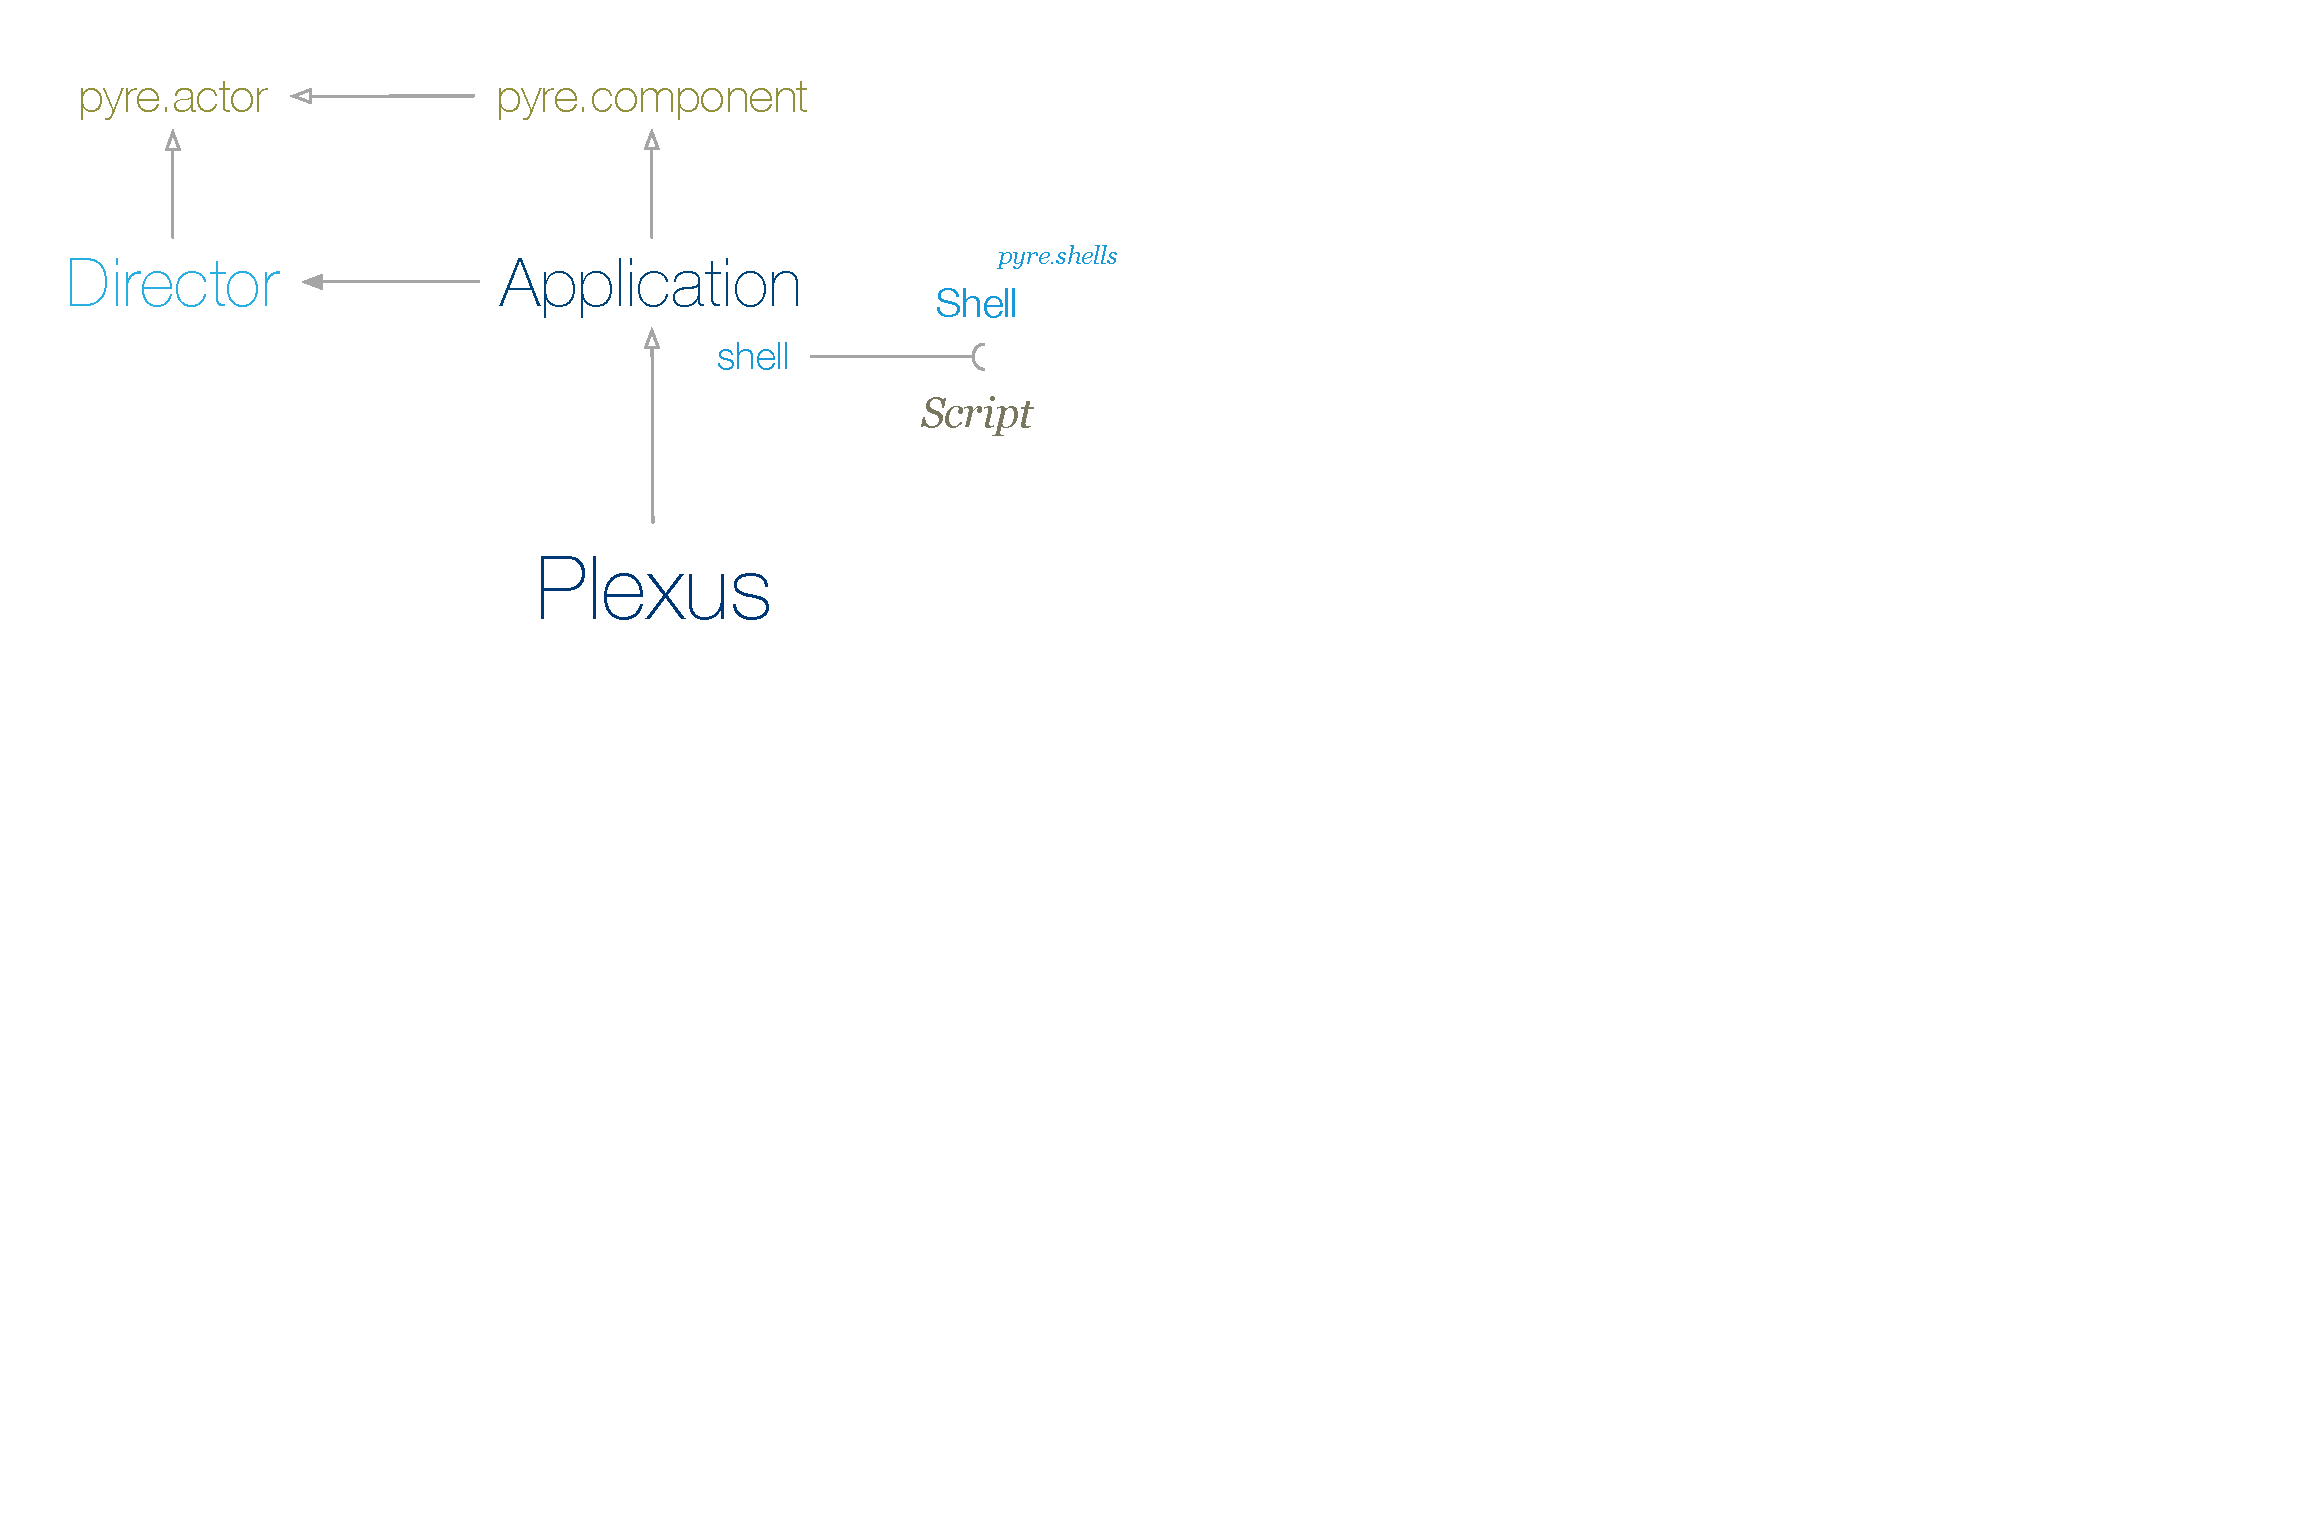
\includegraphics[width=0.9\textwidth]{pyre-plexus-traits}
    \end{center}
  }
  \only<4>{
    \begin{center}
      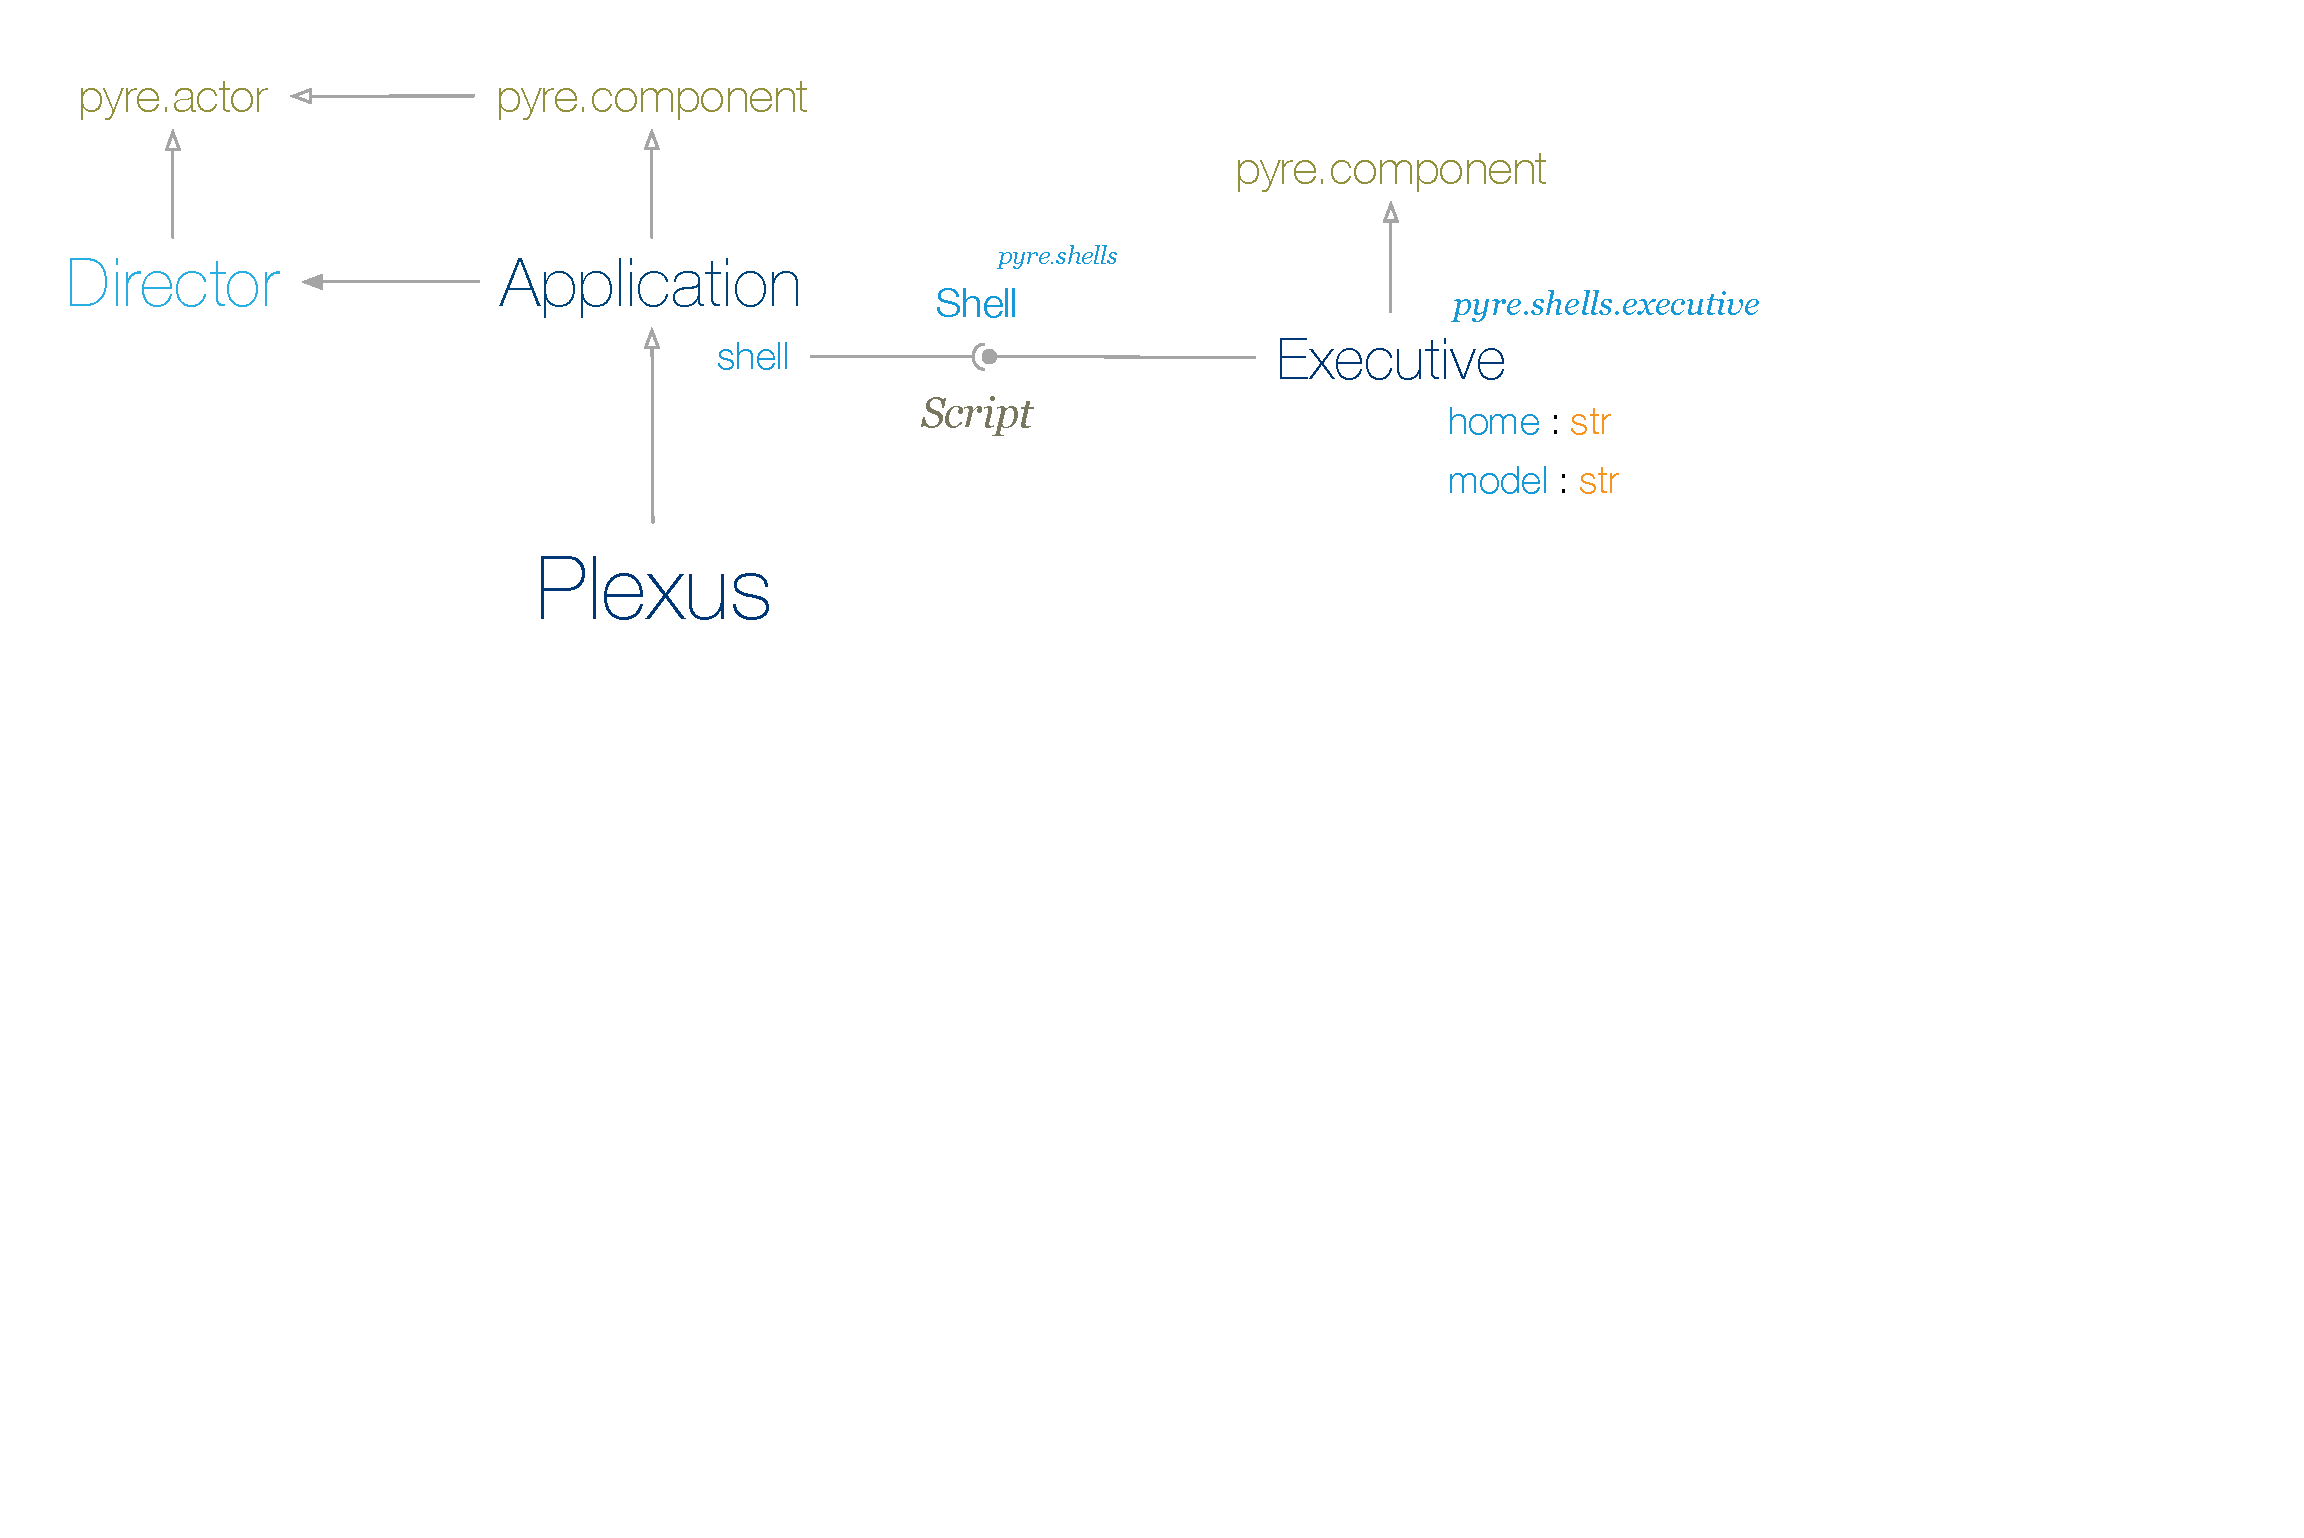
\includegraphics[width=0.9\textwidth]{pyre-plexus-executive}
    \end{center}
  }
  \only<5>{
    \begin{center}
      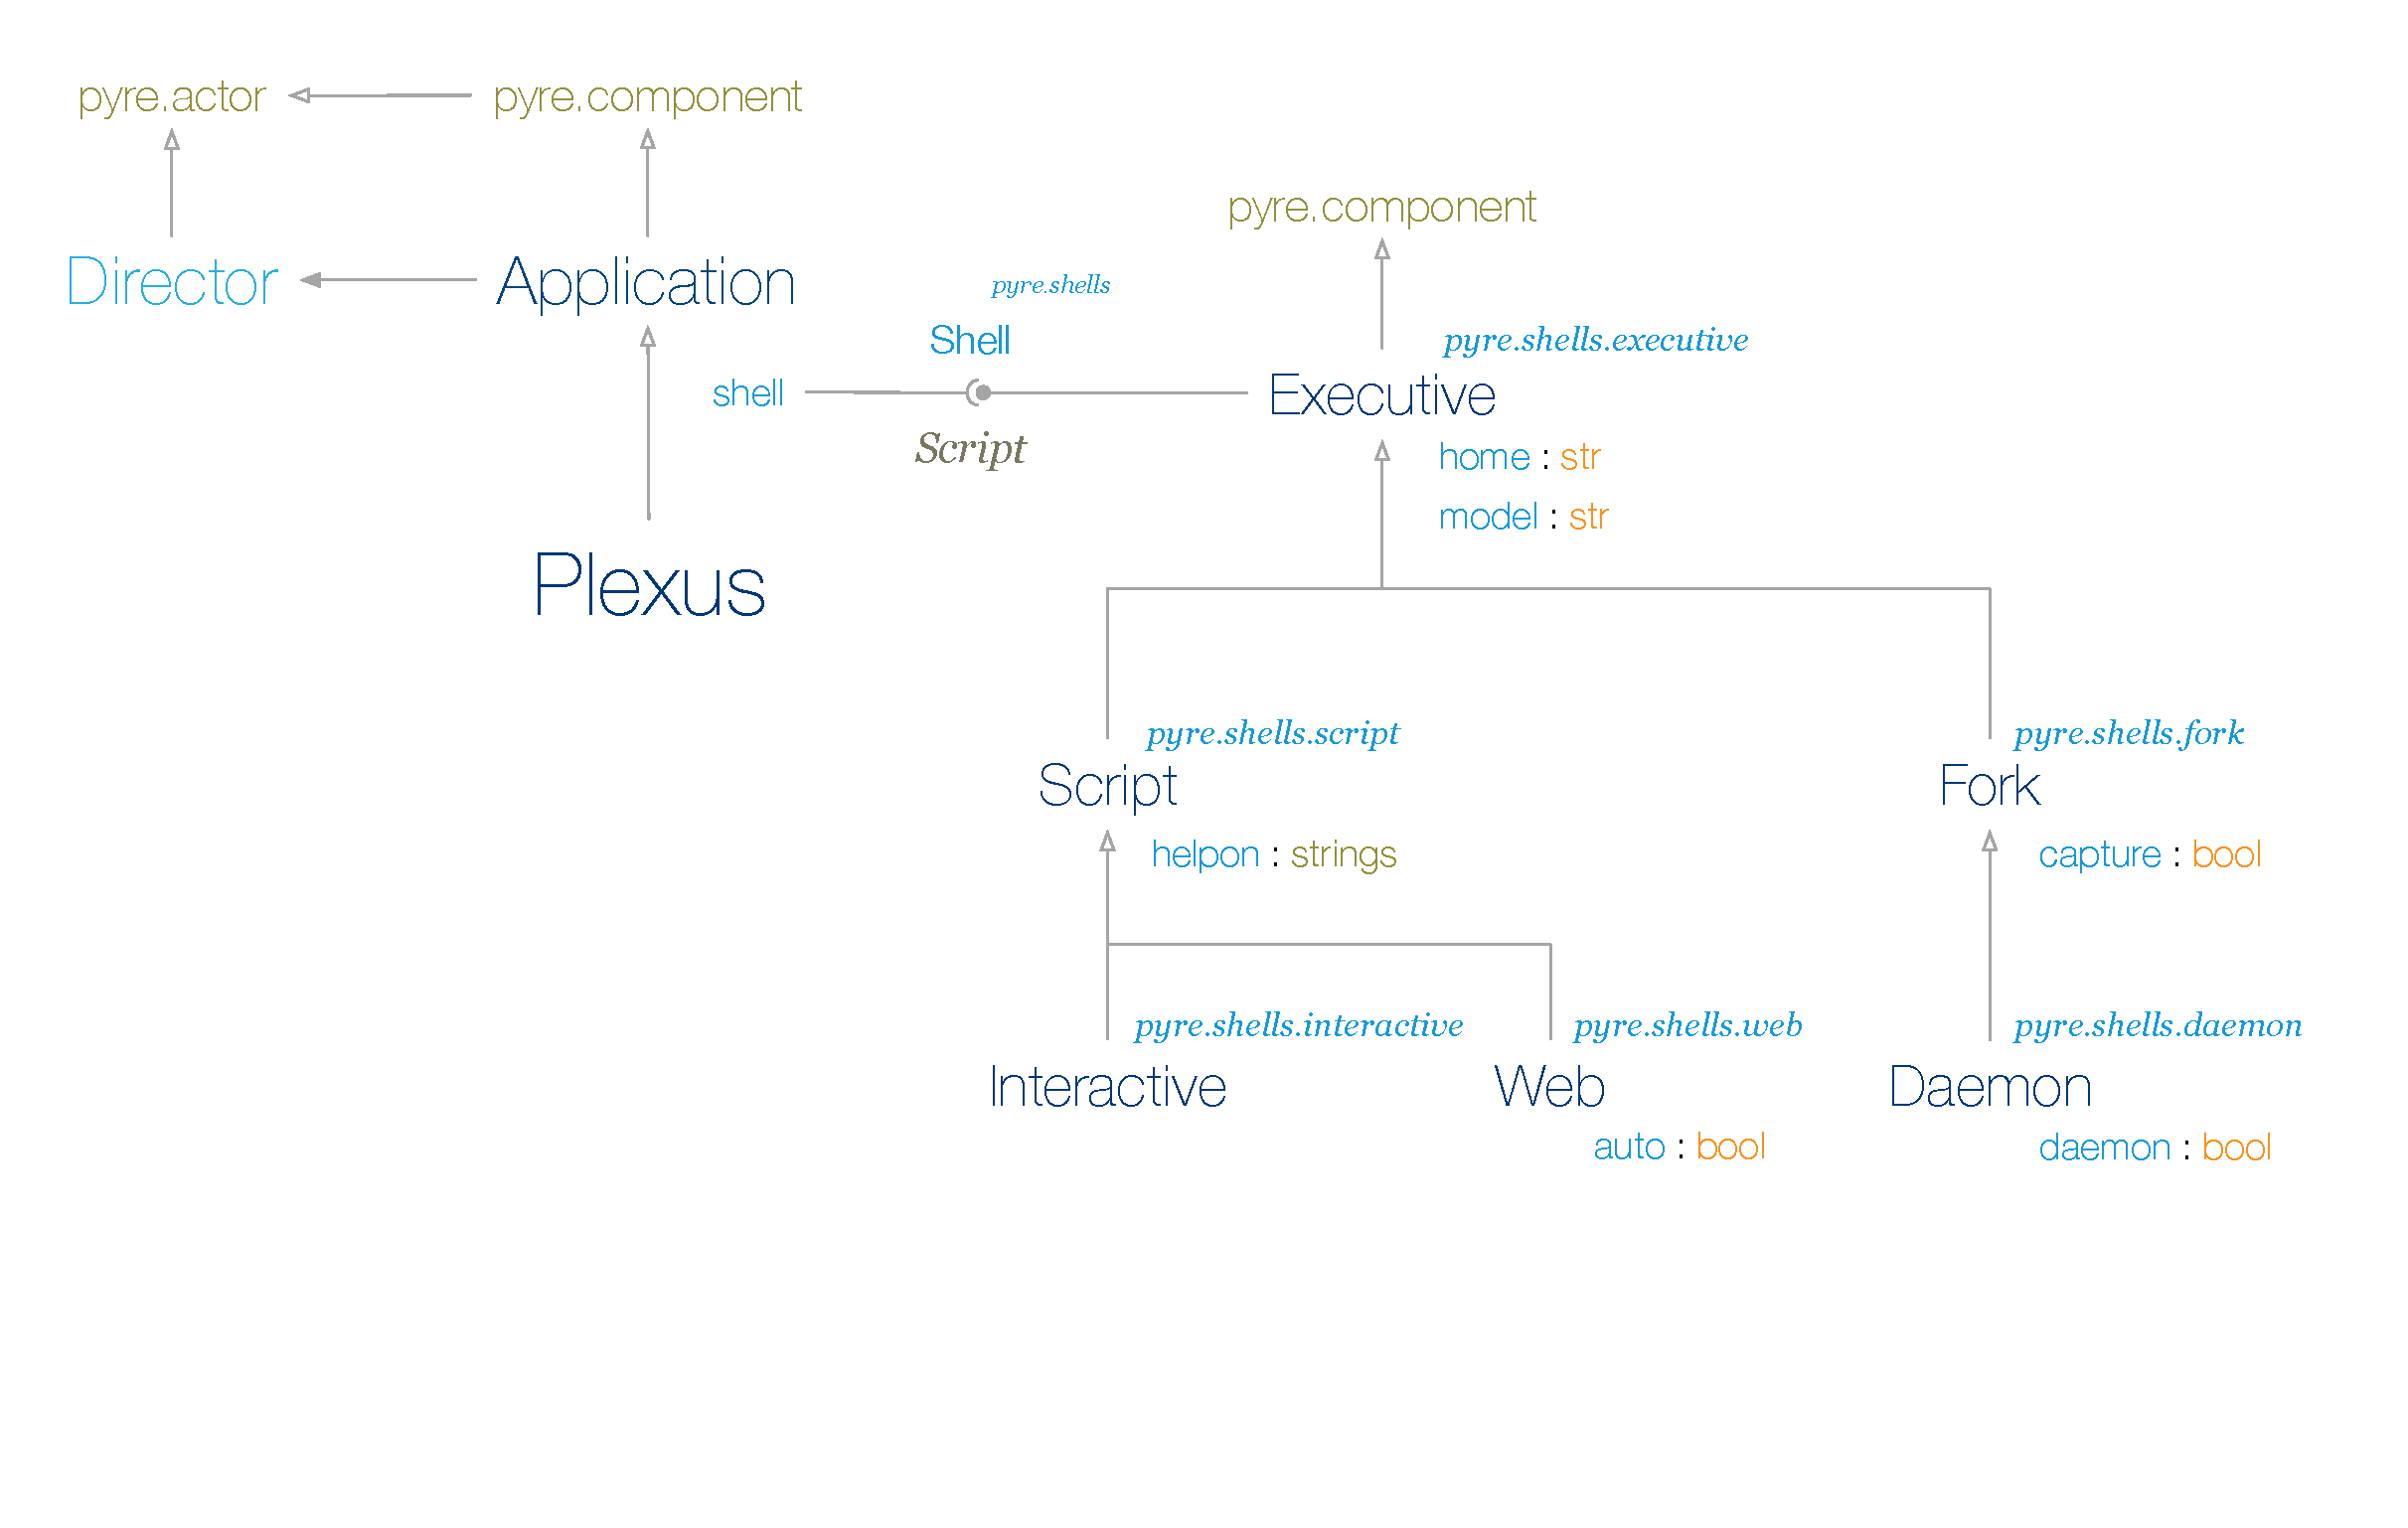
\includegraphics[width=0.9\textwidth]{pyre-plexus-shells}
    \end{center}
  }
  \only<6>{
    \begin{center}
      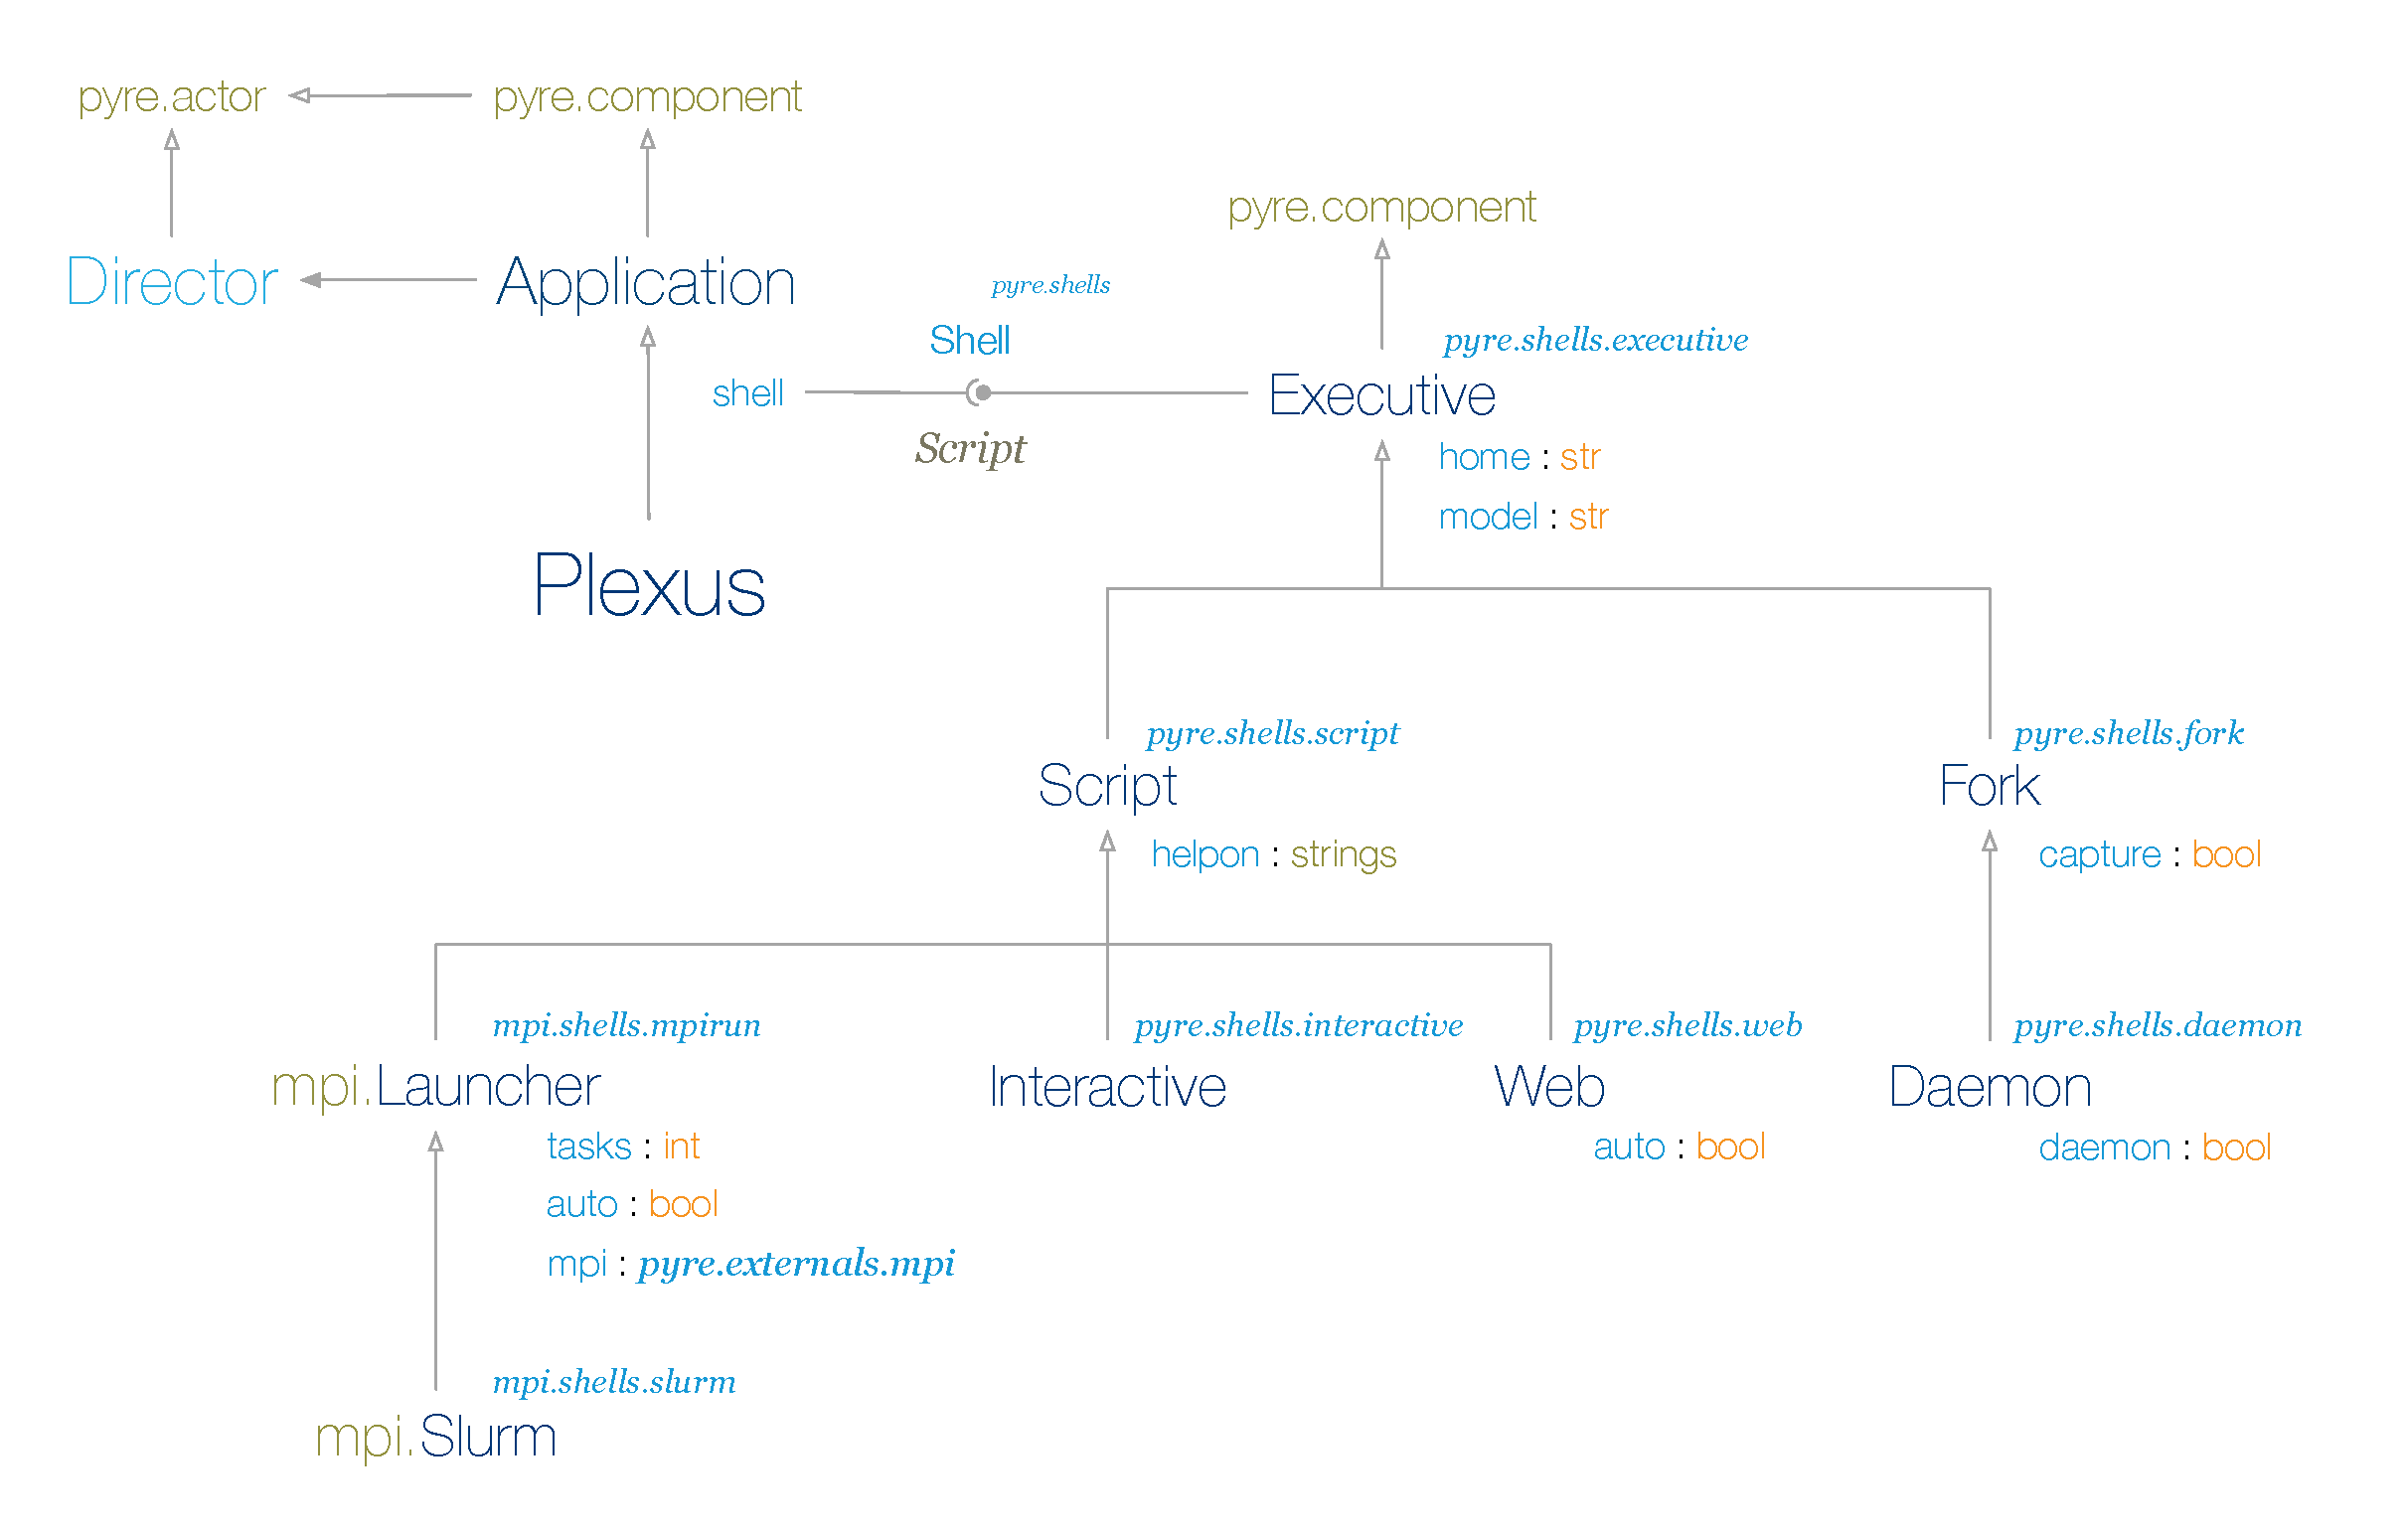
\includegraphics[width=0.9\textwidth]{pyre-plexus-mpi}
    \end{center}
  }
%
\end{frame}

% --------------------------------------

\TODO{
  \item configuration
    \begin{itemize}
    \item conditional assignments
    \item the full assignment uri
    \item assignments involving expressions and references
    \item wiring shortcuts for properly designed package namespaces
    \item having multiple configurations for the same property in the same file
    \item wiring a facility to a specific, perhaps pre\"existing component
    \item syntax rules for each format
    \end{itemize}
  \item explain plexus
  \item convert simple app into a plexus action
  \item more on configuration files
  \item private filesystems
  \item the standard filesystem layout
}


%%% Local Variables:
%%% mode: latex
%%% TeX-master: "../pyre"
%%% End:

% end of file

% -*- LaTeX -*-
% -*- coding: utf-8 -*-
%
% michael a.g. aïvázis <michael.aivazis@para-sim.com>
% (c) 2003-2017 all rights reserved
%

\sectioninlbffalse
\section{to do}

\TODO{
  \item configuration
    \begin{itemize}
    \item the full assignment uri
    \item assignments involving expressions and references
    \item wiring shortcuts for properly designed package namespaces
    \item having multiple configurations for the same property in the same file
    \item wiring a facility to a specific, perhaps pre\"existing component
    \item syntax rules for each format
    \end{itemize}
  \item plexus
    \begin{itemize}
    \item convert simple app into a plexus action
    \end{itemize}
  \item persistence
    \begin{itemize}
    \item filesystem vs.~databases
    \item filesystem abstractions: paths, uris, containers
    \item local, virtual, zip, hdf5, remote
    \item the standard filesystem layout
    \item application private filesystems
    \item databases
    \end{itemize}
  }


%%% Local Variables:
%%% mode: latex
%%% TeX-master: "../pyre"
%%% End:

% end of file


% references
\section{references}
\begin{frame}[allowframebreaks,t]
  \frametitle{References}
  \bibliographystyle{unsrtnat}
  {\footnotesize \bibliography{sections/references}}
\end{frame}

\end{document}

% end of file
